\documentclass[11pt,a4paper,dvipsnames,twosided,final]{article}

\usepackage[deliverable]{IOHKCoverPage}

% data for Deliverable header -- added by KH from an EU H2020 project template
\DeliverableNumber{SL-D4}
\DeliverableTitle{An Introduction to the Shelley Incentives Scheme}{Incentives Scheme Intro.}
\DeliverableResponsible{Formal Methods Team}
\EditorName{Kevin Hammond, \IOHK}
\Authors{Kevin Hammond \quad \texttt{<kevin.hammond@iohk.io>}
}
\DueDate{31$^{\textrm{st}}$ October 2019}
\SubmissionDate{24$^{\textrm{th}}$ October 2019}{2019/10/24}
\LeaderName{Philipp Kant, \IOHK}
\InstitutionAddress{\IOHK}
\Version{0.3}
\Project{Shelley Ledger}
\DisseminationDR

\usepackage[margin=2.5cm]{geometry}
\usepackage{lscape}
\usepackage{iohk}
\usepackage{microtype}
\usepackage{mathpazo} % nice fonts
\usepackage{amsmath}
\usepackage{amssymb}
\usepackage{amsthm}
\usepackage{latexsym}
\usepackage{mathtools}
\usepackage{stmaryrd}
\usepackage{extarrows}
\usepackage{slashed}
%\usepackage[colon]{natbib}
\usepackage[unicode=true,pdftex,pdfa,colorlinks=true]{hyperref}
\usepackage{xcolor}
\definecolor{green}{rgb}{0.0,0.34,0.25}
\usepackage[capitalise,noabbrev,nameinlink]{cleveref}
\usepackage{float}
%\floatstyle{boxed}
\restylefloat{figure}
\usepackage{tikz}
\usepackage{booktabs}
\usepackage{enumerate}

%% Commenting -- KH
\usepackage[obeyFinal]{todonotes}
\newcommand{\khcomment}[1]{\todo[color=blue!20]{KH: #1}}

\newcommand{\ada}{ADA{}}
\newcommand{\ADA}[1]{\textbf{\emph{\ada~{#1}}}}
\newcommand{\cardano}[1]{Cardano}

%% In-para enumeration -- KH
\usepackage{paralist}

\usepackage{caption}

\renewcommand{\floatpagefraction}{0.9}

\begin{document}

\hypersetup{
  pdftitle={},
  breaklinks=true,
  bookmarks=true,
  colorlinks=false,
  linkcolor={blue},
  citecolor={blue},
  urlcolor={blue},
  linkbordercolor={white},
  citebordercolor={white},
  urlbordercolor={white}
}

  \cleardoublepage%
  \tableofcontents%
  \listoffigures%
  \clearpage%

  \begin{changelog}
        \change{2019/10/09}{Kevin Hammond}{FM (\IOHK)}{Initial Version (0.1).}
        \change{2019/10/14}{Kevin Hammond}{FM (\IOHK)}{Version 0.2.  Polished slightly}
        \change{2019/10/15}{Kevin Hammond}{FM (\IOHK)}{First draft of main net calculation.  Fixed small error in Delegator calculation.}
        \change{2019/10/16}{Kevin Hammond}{FM (\IOHK)}{Checked against design document. Further clarifications.}
        \change{2019/10/17}{Kevin Hammond}{FM (\IOHK)}{Further checking and clarification. Added images.}
        \change{2019/10/24}{Kevin Hammond}{FM (\IOHK)}{Version 0.3.  Included images from calculator.  Further checks and improvements.}
      \end{changelog}
      \clearpage%
\begin{landscape}
\floatstyle{plain}
\restylefloat{figure}
\begin{figure*}
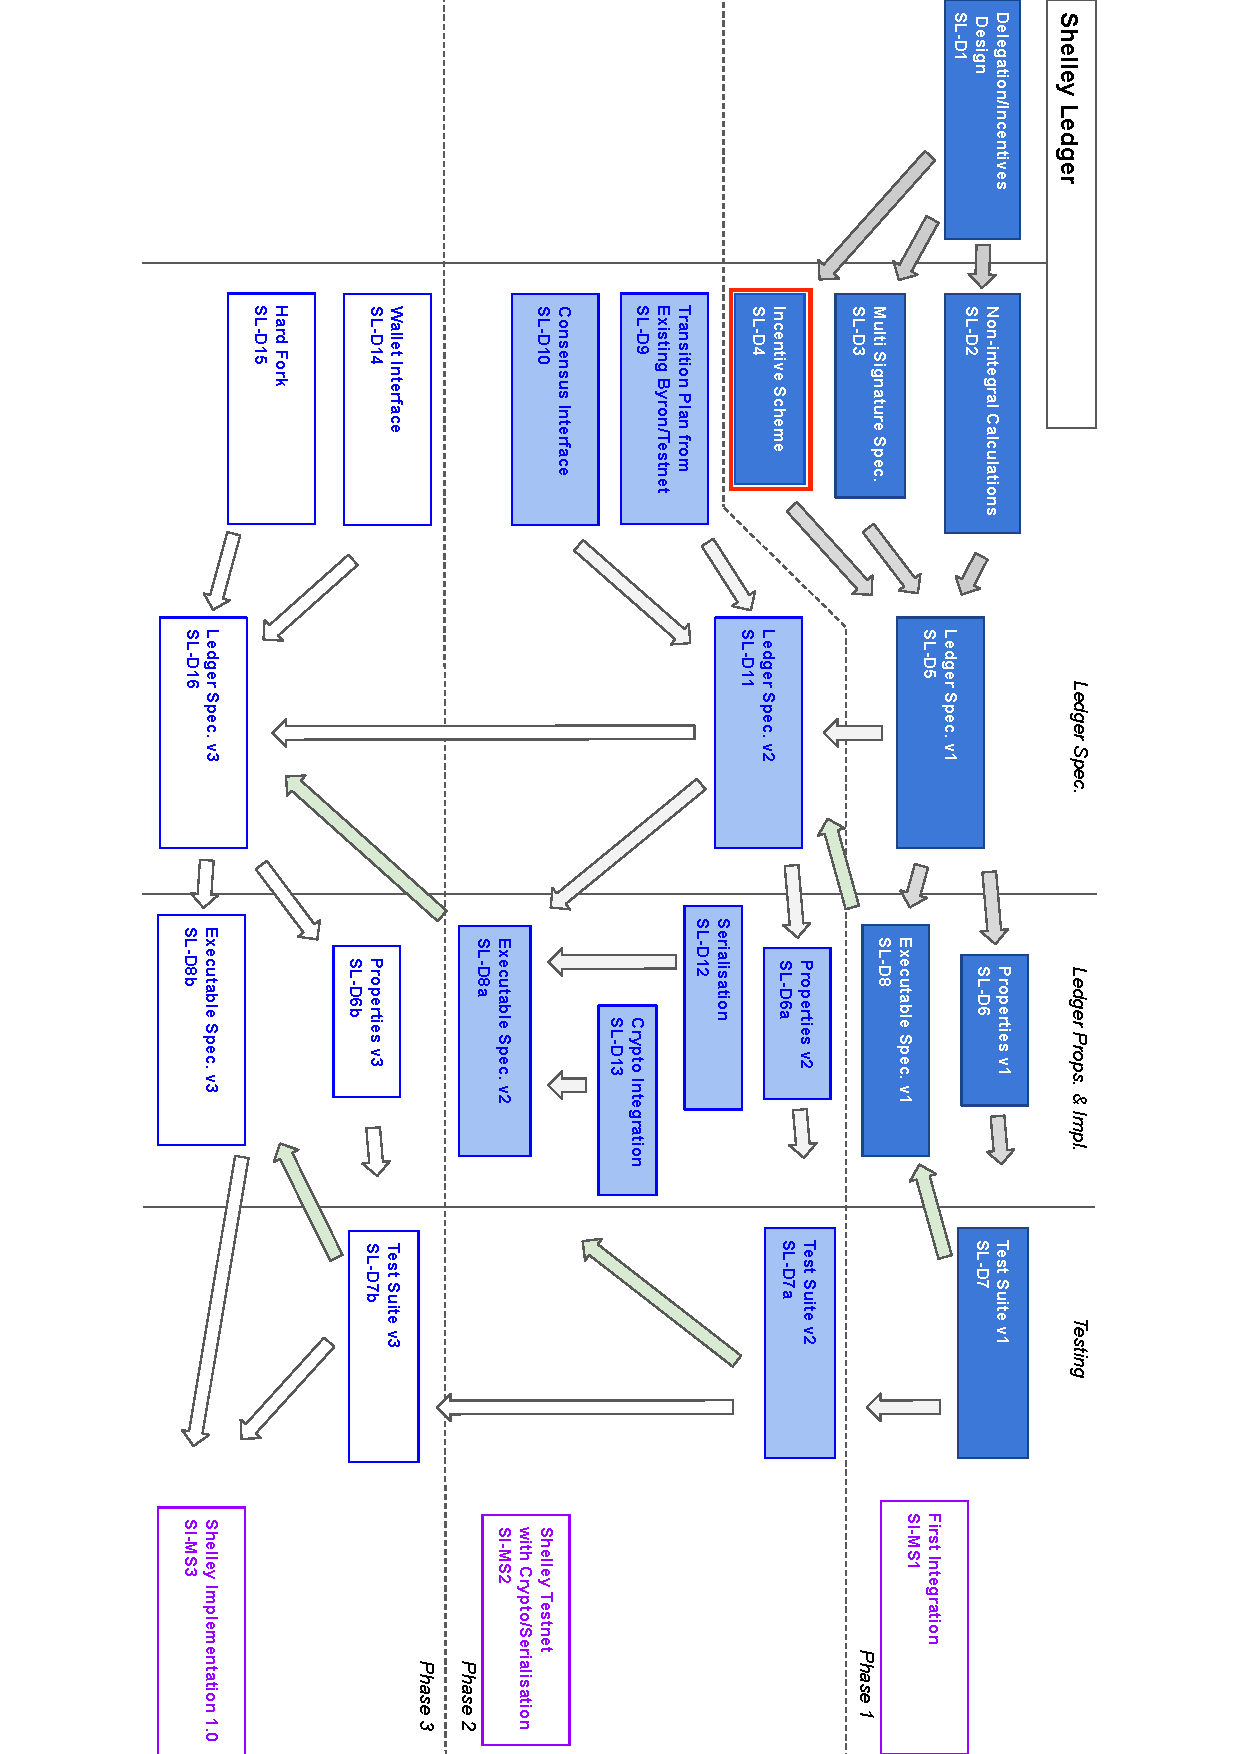
\includegraphics[scale=0.8,angle=90]{d4-depends.pdf}
\caption{Positioning of this Deliverable (outlined in red).}
\end{figure*}
\end{landscape}
%\floatstyle{boxed}
\restylefloat{figure}
\pagestyle{empty}
\cleardoublepage
% \begin{center}
% \large{Executive Summary}
% \end{center}

% \cleardoublepage
% \renewcommand{\thepage}{\arabic{page}}
% \setcounter{page}{1}

\title{An Introduction to the Shelley Incentives Scheme}

\author{Kevin Hammond  \\ {\small \texttt{kevin.hammond@iohk.io}}}

\maketitle

\begin{abstract}
  \noindent
  This document provides a high-level overview of the proposed incentives rewards schemes for
  the Shelley Incentivised TestNet and the subsequent MainNet, highlighting key
  differences between the two schemes.  It is intended to act as a
  simple, easy to follow, guide to the operation of each of the incentives schemes that explains each step of the calculation.
  It assumes a basic familiarity with the concepts of a \emph{blockchain} approach.
  The incentives scheme is designed to ensure the correct operation of the Ouroboros Praos
  protocol, including maintaining built-in defences against ``Sybil-in-Sybil'' security attacks
  that could lead to corruption of the blockchain.  It builds on sound economic theory.
  A simplified version of the incentives scheme is used for the Incentivised TestNet, using fixed rewards,
  omitting fee calculations, StakePool deposits, the influence of the StakePool owner(s)' pledge on
  the StakePool's desirability, the apparent performance of the StakePool etc. (some of these features may be
  added in later versions of the Incentivised TestNet).
  This document is based on SL-D1 (Delegation/Incentives Design)~\cite{delegation_design} and feeds in to SL-D5
  (Formal Ledger Specification. Version 1)~\cite{shelley_spec} as well as the online rewards calculator and the Shelley Incentivised TestNet and MainNet  implementations and quality assurance programmes.
\end{abstract}

\vspace{3.5in}
\noindent
%\begin{center}
\textbf{\emph{Note: this document is subject to change.  In particular, it may be necessary to include a simplified fees calculation
    in the incentivised TestNet, where all the fees accrue to the treasury.
Also note that some terms and symbols that were used in SL-D1 have been changed in this document
in order to simplify the explanations that are given here.  These are outlined in Appendix~\ref{app:diffs}.
}}
%\end{center}

\thispagestyle{empty}
\clearpage
\pagestyle{myheadings}
\renewcommand{\thepage}{\arabic{page}}
\setcounter{page}{1}
\section{Introduction}
\label{sec:introduction}

The purpose of this document is to precisely explain the incentives schemes that will be used by the Shelley implementation
of the \cardano{} blockchain, giving step-by-step explanations of the rewards calculations.
It follows Section~5 of SL-D1 (Delegation/Incentives Design)~\cite{delegation_design}, but aims to provide a more approachable
description that can be used by e.g. StakePool owners/operators, delegators etc.
It also explains the differences between the simplified scheme that will be used in the Shelley Incentivised TestNet implementation and the
full scheme that will be used in the Shelley MainNet implementation.

Figure~\ref{fig:terminology} gives some basic terminology that will be used in this document.
The Shelley implementation rewards those \ada{} holders who either own active stake pools
(\emph{Owners}) or who delegate stake to active stake pools (\emph{Delegators}).
In line with the design of the Ouroboros protocol~\cite{ouroboros_classic}, the \emph{StakePool} receives
rewards in proportion to the stake that it \emph{controls} (``proof of
stake'') rather than in proportion to the work that it does (``proof of work'').
This has cost, efficiency and safety advantages.
The rewards scheme is designed to help ensure that no single entity can
dominate the system by \emph{controlling} excessive amounts of \ada{}.  This is achieved by creating intrinsic
balancing mechanisms that will naturally spread all the active stake among a large number of StakePools.
In particular, the rewards to any one \emph{StakePool} may be capped to a pre-determined limit,
meaning that both delegators and owners will receive less reward if too much stake is controlled by a single StakePool,
so encouraging the creation of additional, smaller StakePools.
It is also designed to ensure \emph{non-myopic} behaviour.  That is, it avoids chaotic system behaviour by encouraging the delegation of \ada{} to those StakePools that will provide
the best overall returns over an extended period of time rather than over the short term.
% This includes limiting the amount of \ada{} that is delegated to any one \emph{StakePool}.
The overall theory that ensures this is described in the Ouroboros Praos research
paper~\cite{ouroboros_praos}; Section~5 of SL-D1~\cite{delegation_design} provides the design rationale
for the actual incentives scheme.

\begin{figure}[t]
  \begin{center}
\begin{tabular}{||l|p{12cm}||}
  \hline \hline
\textbf{Term} & \textbf{Definition} \\\hline
  StakePool & A system that is actively participating in the creation of blocks on the \cardano{} blockchain  \\\hline
  Stake & An amount of \ada{} that is \emph{controlled} by a StakePool.\\\hline
  Epoch & A fixed period of time during which blocks are created, transactions run, and rewards earned.\\\hline
Operator & The entity that is responsible for running a StakePool. \\\hline
Owner(s) & The entities that \emph{pledge} stake to the StakePool when it is registered. \\\hline
  Delegator(s) & The entities that \emph{delegate} stake to the StakePool.\\\hline
  Treasury & A Central Repository of \ada{} to be distributed in future.\\\hline
  Reserve & The \ada{} that is not yet in circulation.\\\hline
  Distribution & The \ada{} that put into circulation in an Epoch.\\\hline
  Reward & The \ada{} that is distributed to the Owner(s) and Delegator(s) of a sufficiently performant StakePool.\\\hline
  MainNet & The full Shelley \cardano{} implementation.\\\hline
  \hline
\end{tabular}
\end{center}
\caption{General Terminology}
\label{fig:terminology}
\end{figure}

\newpage
\subsubsection*{Notation}

Throughout the document, the colour coding below is used to distinguish the sources of various parameters.
A similar scheme is followed in the corresponding spreadsheets.

\begin{tabular}{||l|l||}\hline\hline
  \textbf{\color{green} Green} & Parameters that are set by the \cardano{} system \\\hline
  \textbf{\color{red} Red} & Parameters that are set by a StakePool's Owner(s)/Operator \\\hline
  \textbf{\color{blue} Blue} & Parameters that are set externally \\\hline
  \textbf{\color{cyan} Cyan} & Parameters that are observed from the running implementation \\\hline
  Black & Calculated parameters \\\hline
\hline
\end{tabular}

\subsection{General Parameters}

\begin{figure}[h!]
\begin{center}
\begin{tabular}{||l|l|p{10cm}|l||}
  \hline \hline
\textbf{Parameter} & \textbf{Expected Value} & \textbf{Definition} \\\hline
\textbf{\color{green} \emph{k}} &\textbf{\color{green}  50-1000} & \textbf{\color{green} The Target Number of StakePools} \\\hline
\textbf{\color{green} $T$ } & \textbf{\color{green}  10\% } & \textbf{\color{green}  The Treasury Top Slice Percentage } \\\hline
\textbf{\color{green} $\textit{MER}$ } & \textbf{\color{green}  10\%-15\% } & \textbf{\color{green}   The ``Monetary Expansion Rate'' per Year } \\\hline
\textbf{\color{green} $\textit{DPE}$ } & \textbf{\color{green}  1-5 } & \textbf{\color{green}   Days per Epoch: Duration of a \cardano{} Epoch } \\\hline
  \hline
\end{tabular}
\end{center}
\caption{Key Operational Parameters.}
\end{figure}

\noindent
Four key operating parameters are set by the community (the initial values will be determined by \IOHK):
$k$, the target number of StakePools;
$T$, the treasury top slice percentage;
$\textit{MER}$, the monetary expansion per year;
and
$\textit{DPE}$, the length of each epoch, in days.
%
The target number of StakePools is used to cap the rewards that any individual StakePool can receive. The intention is to encourage the creation of more StakePools, and to avoid domination by any single stake holder.
The \emph{treasury top slice percentage} is the fraction of reward that is allocated to the treasury to cover fixed operating costs, and
ensure the long-term viability both of \cardano{} and of \ada{} as a currency.  It is initially set to a small percentage (10\%) of the rewards.
The \emph{monetary expansion rate} is the rate at which rewards are allocated from the \emph{reserves} of \ada{}.

\begin{figure}[h!]
\begin{center}
\begin{tabular}{||l|l|p{6cm}|l||}
  \hline \hline
\textbf{Parameter} & \textbf{Value} & \textbf{Description} & \textbf{Calculated as} \\\hline
\textbf{\color{blue} $\textit{Ada}^{Tot}$ } & \textbf{\color{blue}  \ADA{45bn} } & \textbf{\color{blue}  The total \ada{} that could ever be created } & \textbf{\color{blue}  } \\\hline
\textbf{\color{blue} \emph{P} } & \textbf{\color{blue}  20\%-50\% } & \textbf{\color{blue}  Participation Rate in the Shelley Incentivised TestNet } & \textbf{\color{blue}  } \\\hline
\textbf{\color{blue} $\textit{Ada}^{\textit{Circ}}$ } & \textbf{\color{blue}  \ADA{31bn} } & \textbf{\color{blue}  The total \ada{} in circulation at Shelley launch } & \textbf{\color{blue}  } \\\hline
\textbf{\color{blue} $\textit{Ada}^{\textit{Rsv}}$ } & \textbf{\color{blue}  \ADA{14bn} } & \textbf{\color{blue}  The total \ada{} in the reserves at Shelley launch } & \textbf{\color{blue}  $\textit{Ada}^{Tot} - \textit{Ada}^{\textit{Circ}}$ } \\\hline
\hline
\end{tabular}
\end{center}
\caption{Parameters that are set by External Factors (e.g. \ada{} holders).}
\end{figure}

\noindent
Several parameters are pre-determined by external factors. These include the
total \ada{} that could ever be created, $\textit{Ada}^{Tot}$;
the total \ada{} that is in \emph{circulation} when the Shelley system launches
(i.e. all \ada{} that is held by any entity on the launch date), $\textit{Ada}^{\textit{Circ}}$;
and the \ada{} that is held in reserve when the system starts.
These values are fixed and will not change.

%\clearpage
\subsection{StakePools}

\subsubsection*{Operator-Set Parameters}

\begin{figure}[h!]
\begin{center}
\begin{tabular}{||l|l|p{9cm}||}
  \hline \hline
\textbf{Parameter} & \textbf{Range} & \textbf{Description} \\\hline
       \textbf{\color{red} $\textit{Pool}^{\textit{Cost}}$} &  \textbf{\color{red}  \ADA{0} $\ldots$} & \textbf{\color{red} Cost
         \emph{per day} in \ada{}} \\\hline
\textbf{\color{red} ${\textit{Pool}}^{\textit{Margin}}$} &  \textbf{\color{red} 0\%-100\%} & \textbf{\color{red} Percentage fee on rewards (the ``margin'')} \\\hline
  \hline
\end{tabular}
\end{center}
\caption{Key Parameters that are set by the StakePool Operator.}
\end{figure}

\noindent
The two main parameters that need to be set by the StakePool \emph{Operator} are the cost \emph{per day} that will be charged to
the pool (in \ada), $\textit{Pool}^{\textit{Cost}}$; and the percentage of any rewards that will subsequently be taken as a fee, ${\textit{Pool}}^{\textit{Margin}}$.
The cost is subtracted from the total rewards that are earned by the pool before any rewards are distributed.
These parameters are advertised by the StakePool and used as part of the public ranking scheme.

\subsubsection*{Sources of Rewards}

Rewards are taken from three sources:

\begin{enumerate}
\item
  monetary expansion (Section~\ref{sec:expansion});
\item
  transaction fees (Section~\ref{sec:fees});
\item
  non-refundable deposits.
\end{enumerate}

\noindent
In the Incentivised TestNet, only the first source is likely to be used.

\subsubsection*{The Rewards that are received by a StakePool}

The rewards that are received by a StakePool will be proportional to the total amount of \ada{} that it controls
as a fraction of the total \ada{} that is in circulation.  The \emph{treasury top slice} is deducted from the total \emph{distribution}
in an epoch, then the remainder plus any fees is distributed proportionately to each StakePool.  In order to avoid domination by large StakePools,
a rewards \emph{cap} will be applied to any single pool, based on the target number of StakePools, $k$.
This is described in more detail in Sections~\ref{sec:TestNet} and~\ref{sec:MainNet}.
% \khcomment{Check: fees before or after cap?} Before, as described

\clearpage
\begin{figure}[h!]
\begin{center}
\begin{tabular}{||l|p{9cm}|l||}
  \hline \hline
\textbf{Parameter} & \textbf{Description} & \textbf{Calculated as} \\\hline
\textbf{\color{red} ${\textit{Pool}}^\textit{Pledge}$} & \textbf{\color{red} \ada{} that is pledged to the StakePool by the Owner(s)} & \\\hline
\textbf{\color{blue} ${\textit{Pool}}^\textit{Deleg}$} & \textbf{\color{blue}  \ada{} that is delegated to the StakePool} & \\\hline
${\textit{Pool}}^{Tot}$ & All \ada{} that is controlled by the StakePool & ${\textit{Pool}}^\textit{Pledge} + {\textit{Pool}}^\textit{Deleg}$ \\\hline
${\textit{Pool}}^\%$ & Fraction of the \ada{} in circulation that is controlled by the StakePool & {\large $\frac{{\textit{Pool}}^{Tot}}{\textit{Ada}^{\textit{Circ}}}$} \\\hline
  \hline
\end{tabular}
\end{center}
\caption{The \ada{} that is controlled by a StakePool.}
\end{figure}

\noindent
The total \ada{} that a StakePool controls is the sum of the \ada{} that is \emph{pledged} to the StakePool by the owners(s) plus
the additional \ada{} that is \emph{delegated} to the StakePool.  An owner may \emph{delegate} to a StakePool if
they wish as well as \emph{pledging} to it, but would receive lower rewards for their \emph{delegated} stake.
In return for receiving higher rewards, \emph{pledging} incurs higher risk, requiring owners to \emph{trust} each other.


\subsubsection*{The Rewards that are given to Owner(s) and Delegators}

Once the pool operating charges are subtracted from the net rewards, any remaining reward is distributed to the owner(s) and delegators
in proportion to their pledged/delegated stake.  The Incentivised TestNet uses a simplified scheme for the owner reward calculations.


\clearpage
\section{The Simplified Incentives Scheme (Shelley Incentivised TestNet)}
\label{sec:TestNet}

The simplified scheme calculates rewards based on the total number of blocks that each stake pool produces,
and distributes a fixed amount of \ada{} per epoch.
Since \cardano{} is based on \emph{proof of stake}, then on average, each stake pool will obtain
rewards that are proportional to the stake that it holds.  So, if e.g. a pool holds 1\% of the total
\ada{} in circulation, then it will receive, on average, 1\% of the total rewards that are allocated to all the
StakePools.

\begin{figure}[h!]
\begin{center}
\begin{tabular}{||l|l|p{10cm}|l||}
  \hline \hline
\textbf{Parameter} & \textbf{Expected Value} & \textbf{Definition} \\\hline
\textbf{\color{green} \emph{k}} & \textbf{\color{green} 50-100} &\textbf{\color{green}  The Target Number of StakePools} \\\hline
\textbf{\color{green} $T$} & \textbf{\color{green} 10\%} & \textbf{\color{green} The Treasury Top Slice Percentage} \\\hline
\textbf{\color{green} $\textit{MER}$} & \textbf{\color{green} 10\%}&  \textbf{\color{green} The ``Monetary Expansion Rate'' per Year}\\\hline
\textbf{\color{green} $\textit{DPE}$} & \textbf{\color{green} 1} & \textbf{\color{green}  Days per Epoch: Duration of a \cardano{} Epoch} \\\hline
  \hline
\end{tabular}
\end{center}
\caption{Settings for Key Operational Parameters in the Incentivised TestNet.}
\end{figure}

\noindent
In the Incentivised TestNet,
the target number of StakePools, \emph{k} is expected to be 50-100 initially, but this will be increased as necessary to encourage the creation of more StakePools.
In the MainNet, it is expected to rise over time, up to about 1000.
The treasury top slice percentage, $T$ is fixed at 10\% of the total distribution per epoch (this is expected to be unchanged in the MainNet).
The monetary expansion rate, $\textit{Mer}$ is fixed at the equivalent of 10\% per annum, so that precisely 10\% of the \ada{} reserves would be distributed
if the TestNet were to run for one complete year, or precisely 2.5\% of the \ada{} reserves would be distributed if it were to run for 3 months.
For simplicity and to ensure that epoch changes occur frequently, in the Incentivised TestNet, the length of each epoch ($\textit{DPE}$) has been set to 1 day.

\begin{figure}[h!]
\begin{center}
\begin{tabular}{||l|l|p{6cm}|l||}
  \hline \hline
\textbf{Parameter} & \textbf{Expected Value} & \textbf{Description} & \textbf{Calculated as} \\\hline
\textbf{\color{blue} \emph{P}} & \textbf{\color{blue} 20\%-50}\% & \textbf{\color{blue} Participation Rate in the TestNet} & \\\hline
$\textit{Ada}^{\textit{Circ}}_{\textit{Test}}$ & \ADA{15.5bn} @ $P=50\%$ & The \ada{} circulating in the TestNet & $P \times \textit{Ada}^{\textit{Circ}}$ \\\hline
  \hline
\end{tabular}
\end{center}
\caption{\ada{} in Circulation in the Incentivised TestNet.}
\end{figure}

\noindent
The \emph{participation rate} is used to calculate the total amount of \ada{} that will circulate in the Incentivised TestNet.
This rate is simply the percentage of the total \ada{} in  circulation that is available to be staked in the Incentivised TestNet.
It will be determined at the date when the
TestNet launches and will then remain fixed.
% \khcomment{Check - no \ada{} can be transferred later - affects the calculations/reward?}.
It is assumed that this is likely to be 20\%-50\% of the total \ada{} in circulation.


\begin{figure}[h!]
\begin{center}
\begin{tabular}{||l|l|p{6cm}|l||}
  \hline \hline
\textbf{Parameter} & \textbf{Expected Value} & \textbf{Description} & \textbf{Calculated as} \\\hline
% $\textit{DPE}$ & 1 & Days per Epoch in the TestNet & \\\hline
% $\textit{MER}$ & 10\% &  The ``Monetary Expansion Rate'' per Year & \\\hline
$\textit{Distr}_E$ & \ADA{3.84M} & Distribution per Epoch in the TestNet & $\frac{\textit{Ada}^{\textit{Rsv}} \times \textit{MER}}{365 \div \textit{DPE}}$ \\\hline
$T_E$ & \ADA{384K} & Treasury Top Slice per Epoch & $\textit{Distr}_E \times T$ \\\hline
$R_E$ & \ADA{3.45M} & Total Rewards per Epoch & $\textit{Distr}_E - T_E$ \\\hline
  \hline
\end{tabular}
\end{center}
\caption{Total Distribution and Rewards per Epoch.}
\label{fig:distrib}
\end{figure}

\noindent
The total \ada{} that is distributed per epoch in the Incentivised TestNet (${\textit{Distr}}_E$) is calculated from the initial
value of the \ada{} reserves, $\textit{Ada}^{\textit{Rsv}}$, and the fixed monetary expansion rate, \textit{MER}.
An equal distribution is given per epoch.  The top slice that is allocated to the treasury ($T_E$) is
deducted from this distribution, and the remainder is then allocated to the StakePools as rewards ($R_E$).

\subsubsection*{Transaction Fees in the Incentivised TestNet (possible addition)}

Transaction fees are not considered initially in the Incentivised TestNet, but, if they are eventually included, would simply be allocated to
the Treasury.

% \begin{itemize}
%   \i
%   be added to the total distribution, $\textit{Distr}_E$, before deducting the Treasury Top Slice:
% $\textit{Distr}'_E = \textit{Distr}_E + \textit{Fees}_E$,

%\clearpage
\subsection{The Rewards that are received by a StakePool per Epoch}

\begin{figure}[h!]
\begin{center}
\begin{tabular}{||l|l|p{6cm}|l||}
  \hline \hline
\textbf{Parameter} & \textbf{Expected Value} & \textbf{Definition} & \textbf{Calculated as} \\\hline
  \textbf{\color{red} $\textit{\textit{Pool}}^{\textit{Cost}}$} &  & \textbf{\color{red} Cost per day in \ada{}} & \\\hline
\textbf{\color{red} ${\textit{Pool}}^{\textit{Margin}}$} &  \textbf{\color{red} 0\%-100\%} & \textbf{\color{red} Percentage fee on rewards (the ``margin'')} & \\\hline
\textbf{\color{red} ${\textit{Pool}}^\textit{Pledge}$} & & \textbf{\color{red} \ada{} that is pledged to the StakePool by the Owner(s)} & \\\hline
\textbf{\color{blue} ${\textit{Pool}}^\textit{Deleg}$} & & \textbf{\color{blue} \ada{} that is delegated to the StakePool} & \\\hline
${\textit{Pool}}^{Tot}$ & & All \ada{} that is controlled by the StakePool & ${\textit{Pool}}^\textit{Pledge} + {\textit{Pool}}^\textit{Deleg}$ \\\hline
  ${\textit{Pool}}^\%$ & & Fraction of the \ada{} in circulation that is controlled by the StakePool & {\large $\frac{{\textit{Pool}}^{Tot}}{\textit{Ada}^{\textit{Circ}}_{\textit{Test}}}$} \\\hline
&&&  \\\hline
\textbf{\color{cyan} \emph{N}} & & \textbf{\color{cyan} The Number of Blocks that were allocated to the StakePool} & \\\hline
\textbf{\color{cyan} \emph{n}} & & \textbf{\color{cyan} The Number of Blocks actually Produced by the StakePool} & \\\hline
\emph{p} & & The Performance of the StakePool & $\frac{n}{N}$ \\\hline
\textbf{\color{green} \emph{k}} &\textbf{\color{green} 50-1000} & \textbf{\color{green} The Target Number of StakePools} & \\\hline
\emph{z} & 0.001-0.02 & The Rewards Limit Fraction & $\frac{1}{k}$ \\\hline
\hline
\end{tabular}
\end{center}
\caption{Parameters Governing the Rewards to a StakePool.}
\label{fig:rewards}
\end{figure}

\noindent
The parameters governing the StakePool reward calculation are shown above.  The only new
parameters are $n$, $N$ and $z$. $n$ and $N$ are measured by the system; $z$ is calculated from the
target number of StakePools, $k$.  These parameters limit the rewards that can be received by any StakePool.
% \khcomment{Check that $\textit{Ada}^{\textit{Circ}}_{\textit{Test}}$ is a fixed value.}

\clearpage
\begin{figure}[h!]
\begin{center}
\begin{tabular}{||l|p{7.8cm}|l||}
  \hline \hline
\textbf{Parameter}  & \textbf{Definition} & \textbf{Calculated as} \\\hline
$R^{Gross'}$ & The Average Gross Reward to the StakePool & $R_E \times \textrm{min} (z,{\textit{Pool}}^\%)$ \\\hline
$R^{\textit{Gross}}$ & The Actual Gross Reward to the StakePool & $R^{Gross'} \times \textrm{min} (100\%,p$ \\\hline
${\textit{Pool}}^{\textit{Cost}}_E$ & \textit{Pool} Operator Costs for the Epoch & $\textrm{min}((\textit{\textit{Pool}}^{\textit{Cost}} \times \textit{DPE}),R^{\textit{Gross}})$ \\\hline
$R^{\textit{Net}}$  & The Net Reward to the StakePool & $R^{\textit{Gross}} - {\textit{Pool}}^{\textit{Cost}}_E$ \\\hline
$R^{Owner}$ & The Total Reward to the Owner(s) & $R^{\textit{Net}} \times {\textit{Pool}}^{\textit{Margin}} $ \\\hline
$R^{Deleg}$ & The Total Reward to the Delegators & $R^{\textit{Net}} - R^{Owner}$ \\\hline
$\textit{Owner}^\textit{Income}$ & The Total Pool Owner Income & ${\textit{Pool}}^{\textit{Cost}}_E + R^{Owner}$ \\\hline
\hline
\end{tabular}
\end{center}
\caption{Calculation of the Total Stake Pool Reward.}
\end{figure}

\noindent
The gross reward that is received by the StakePool is, on average, directly proportional to the
stake that it controls, as a proportion of the total \ada{} that is in circulation.
It is limited by the rewards limit fraction, and reduced in proportion to the ratio of blocks that it produced
to the blocks that it was allocated (the ``performance'' of the StakePool) to give $R^{\textit{Gross}}$.
% \khcomment{Check this - not overall performance.}  Checked.
Once the pool operator costs are subtracted,
the net reward is then distributed to the owner(s) and delegators in proportion to the
stake that each group controls.  The StakePool owner income is then the sum of the operator costs and the pool owner rewards.
Note that if there is insufficient gross reward to cover the operator costs, all the reward will be accrued to those
costs, leaving no further reward to be distributed to the either owners or delegators.


\subsubsection*{The Rewards that are received by each Delegator per Epoch}

\begin{figure}[h!]
\begin{center}
\begin{tabular}{||l|p{9cm}|l||}
  \hline \hline
\textbf{Parameter} & \textbf{Definition} & \textbf{Calculated as} \\\hline
${\textit{Pool}}^{Tot}$ & All \ada{} that is controlled by the StakePool & ${\textit{Pool}}^\textit{Pledge} + {\textit{Pool}}^\textit{Deleg}$ \\\hline
$R^{Deleg}$ & The Total Reward to the Delegators & $R^{\textit{Net}} - R^\textit{Owner}$ \\\hline
$D^{Stake}$ & The \ada{} that is delegated by Delegator $D$ & \\\hline
$D^\%$ & The proportion of \ada{} in the StakePool that is delegated by $D$ & $\frac{D^{Stake}}{Pool^{Tot}}$ \\\hline
$D^{Rewards}$ & The \ada{} rewards that are received by $D$ & $R^{\textit{Net}} \times D^\%$ \\\hline
\hline
\end{tabular}
\end{center}
\caption{The Rewards that are received by a specific Delegator, $D$.}
\end{figure}

\noindent
The rewards that are received by an individual delegator are directly proportional to the
stake that the delegator has placed in the StakePool, calculated from the net rewards to the
StakePool.

\clearpage
\subsubsection*{The Rewards that are received by each StakePool Owner per Epoch}

\begin{figure}[h!]
\begin{center}
\begin{tabular}{||l|p{6cm}|l||}
  \hline \hline
\textbf{Parameter}  & \textbf{Definition} & \textbf{Calculated as} \\\hline
$R^\textit{Owner}$ & The Total Reward to the Owner(s) & $R^{\textit{Net}} \times {\textit{Pool}}^{\textit{Margin}} $ \\\hline
$\textit{nOwners}$ & The total number of Owner(s) of the StakePool, $\textit{nOwners} \ge 1$  & \\\hline
$O^{Rewards}$ & The \ada{} rewards that are received by owner $O$ & $R^\textit{Owner} \div \textit{nOwners}$ \\\hline
\hline
\end{tabular}
\end{center}
\caption{The Rewards that are received by a specific Owner $O$.}
\end{figure}

\noindent
In the Incentivised TestNet, the owner rewards are divided equally among the
owners, regardless of the proportion of stake that they pledge.  The assumption
is that, in practice, each owner will pledge an equal amount of stake, but this
is not enforced by the implementation.

%\clearpage
\subsection{Calculating Rewards in External Currencies}
\label{sec:conversion}

\begin{figure}[h!]
\begin{center}
\begin{tabular}{||l|p{6cm}|l||}
  \hline \hline
\textbf{Value} & \textbf{Description} & \textbf{Calculated as} \\\hline
$R_A$ &  Rewards value in \ada{} &\\\hline
$ER_D$ &  Dollar Price per \ada{} &\\\hline
$R_D$ &  Rewards value in dollars & $R_A \times ER_D$ \\\hline
\hline
\end{tabular}
\end{center}
\caption{Calculating Rewards in Terms of Other Currencies}
\label{fig:monetary}
\end{figure}

\noindent
As usual, rewards in \ada{} can easily be converted to an external dollar or other currency equivalent using
the current exchange rate, $ER_D$, as shown % in Figure~\ref{fig:monetary}
above.  For example, if the rewards are \ADA{10,000} and the exchange rate is
\$0.039 (1 \ada{} is worth 3.9 cents).  Realising this value would require the use of an \emph{exchange},
of course.

\clearpage
\subsection{Worked Example: Simplified Scheme}


\begin{minipage}{\textwidth}
  This example is taken from the internal \IOHK{} spreadsheet calculator at
\url{https://docs.google.com/spreadsheets/d/1c-KmCNBIMZjHN7wdsrNx3ac1zT8xEqodK1OyZxC_QIk/edit#gid=1365573139}.
It has been used as the basis for the online calculator at \url{https://cardano-staking-site.netlify.com/en/}.

\subsubsection*{Key Parameters}

\noindent
\vspace{-0.5in}
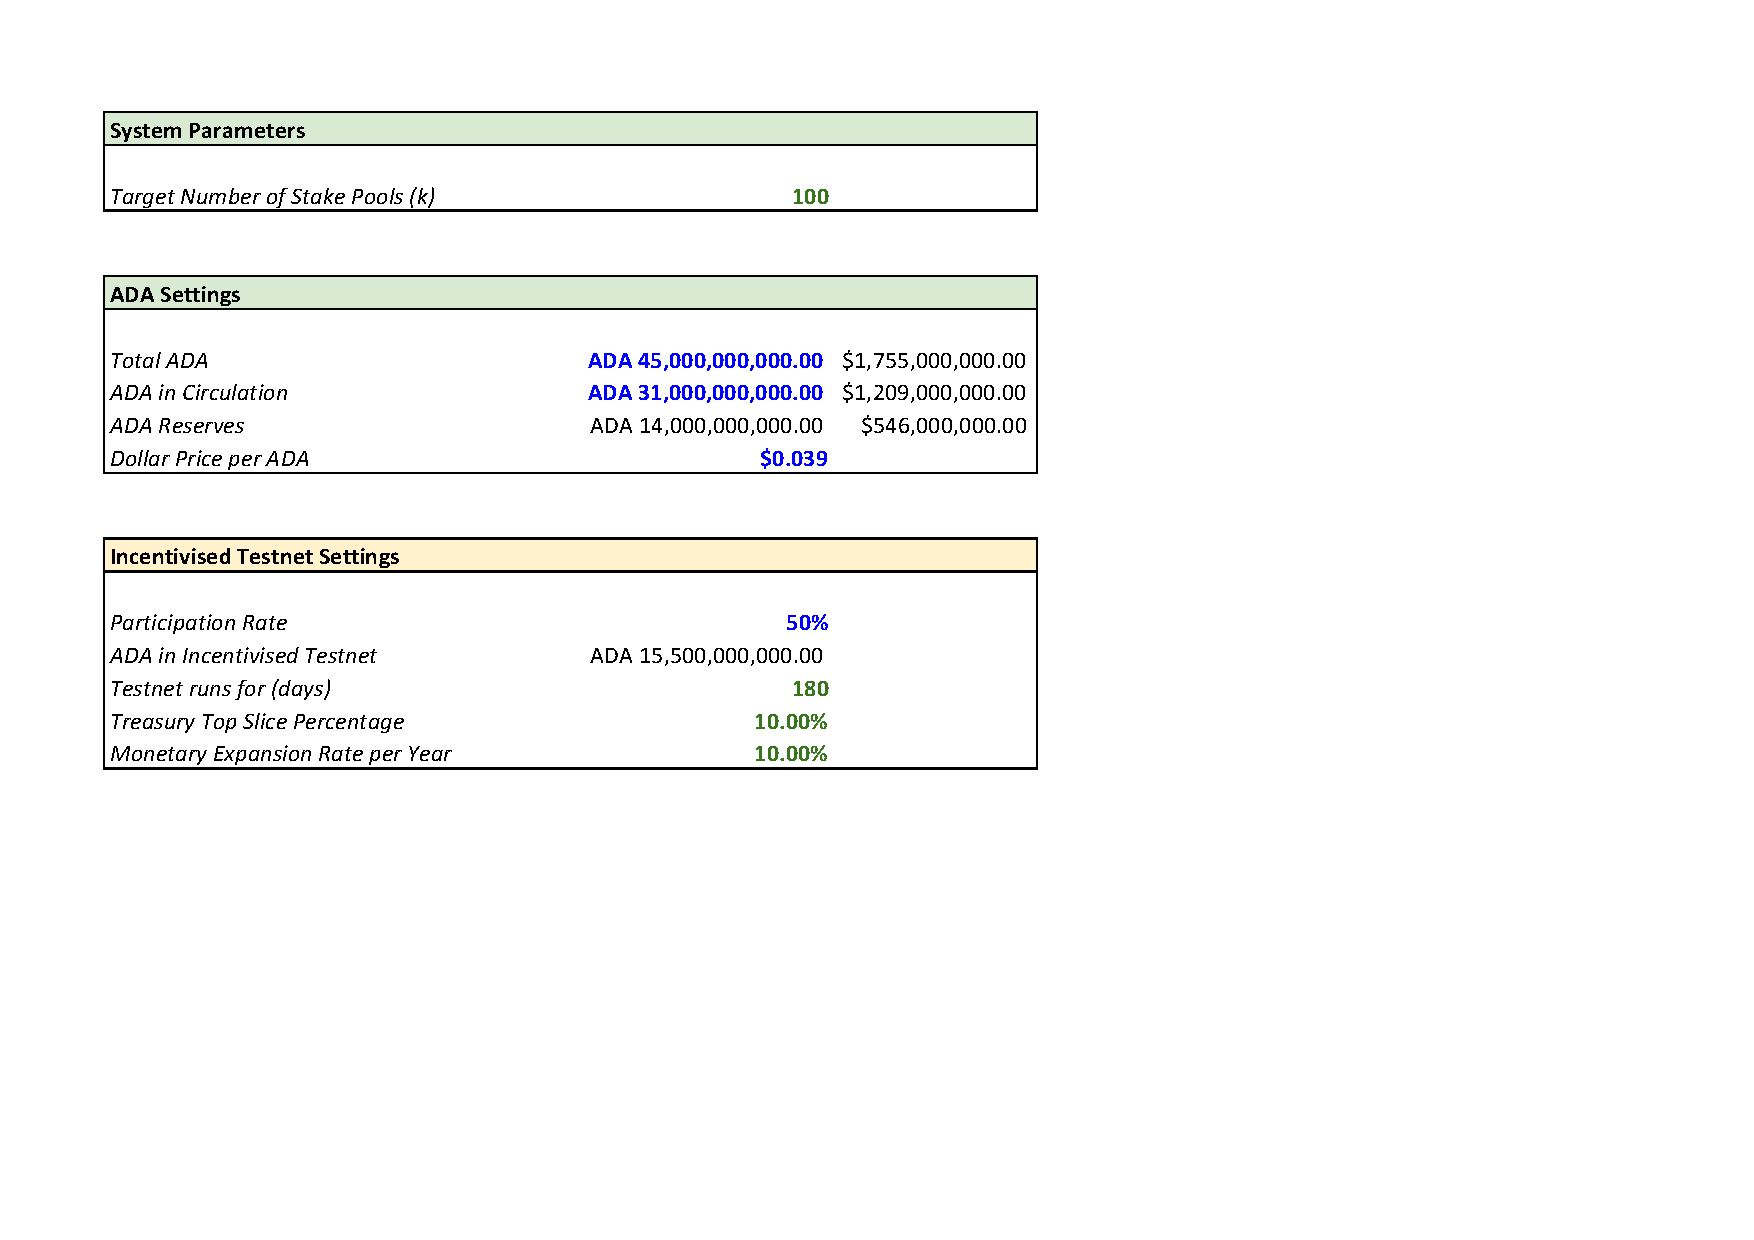
\includegraphics[height=6in]{RCT1.pdf}
\vspace{-2in}

\noindent
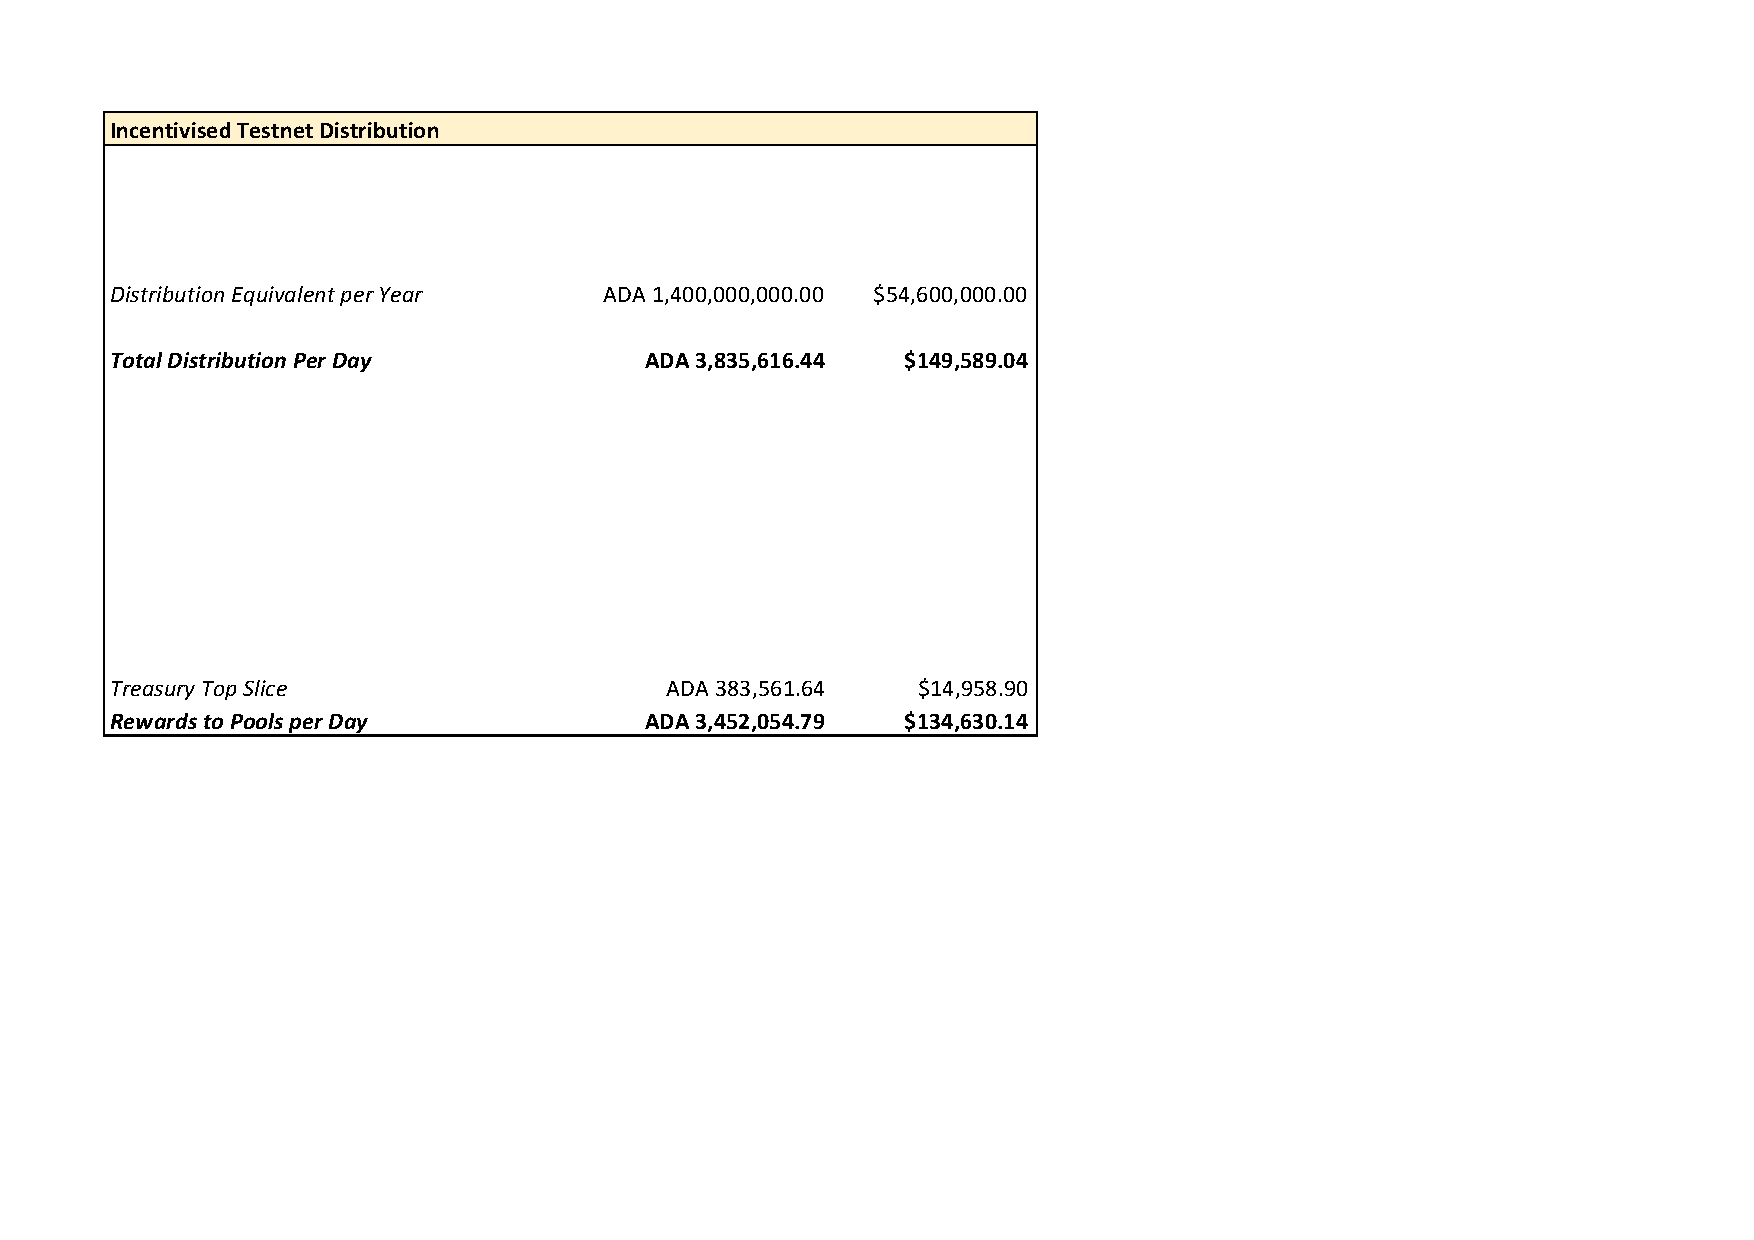
\includegraphics[width=1.2\textwidth]{RCT2.pdf}
\vspace{-1.9in}

\noindent
This diagram shows the key parameters and settings for the rewards system, including the
rewards that are distributed from the reserves at each epoch.  We assume a Treasury Top Slice
of 10\% and the target number of StakePools to be 100.  The \ada{} in circulation and reserves
are the values as of September 24$^{th}$ 2019, rounded to the nearest ADA{1bn}.  We further
assume a \emph{monetary expansion rate} of 10\% and that the TestNet will run for 180 days
(this is used to calculate the initial values of the \ada{} in circulation and in reserve
for the full incentives scheme).  After the Treasury Top Slice is taken, the total
rewards per Epoch (or Day) that will be distributed to the StakePools is \ADA{3,452,054.79}.
\end{minipage}

\clearpage
\subsubsection*{StakePool Parameters}
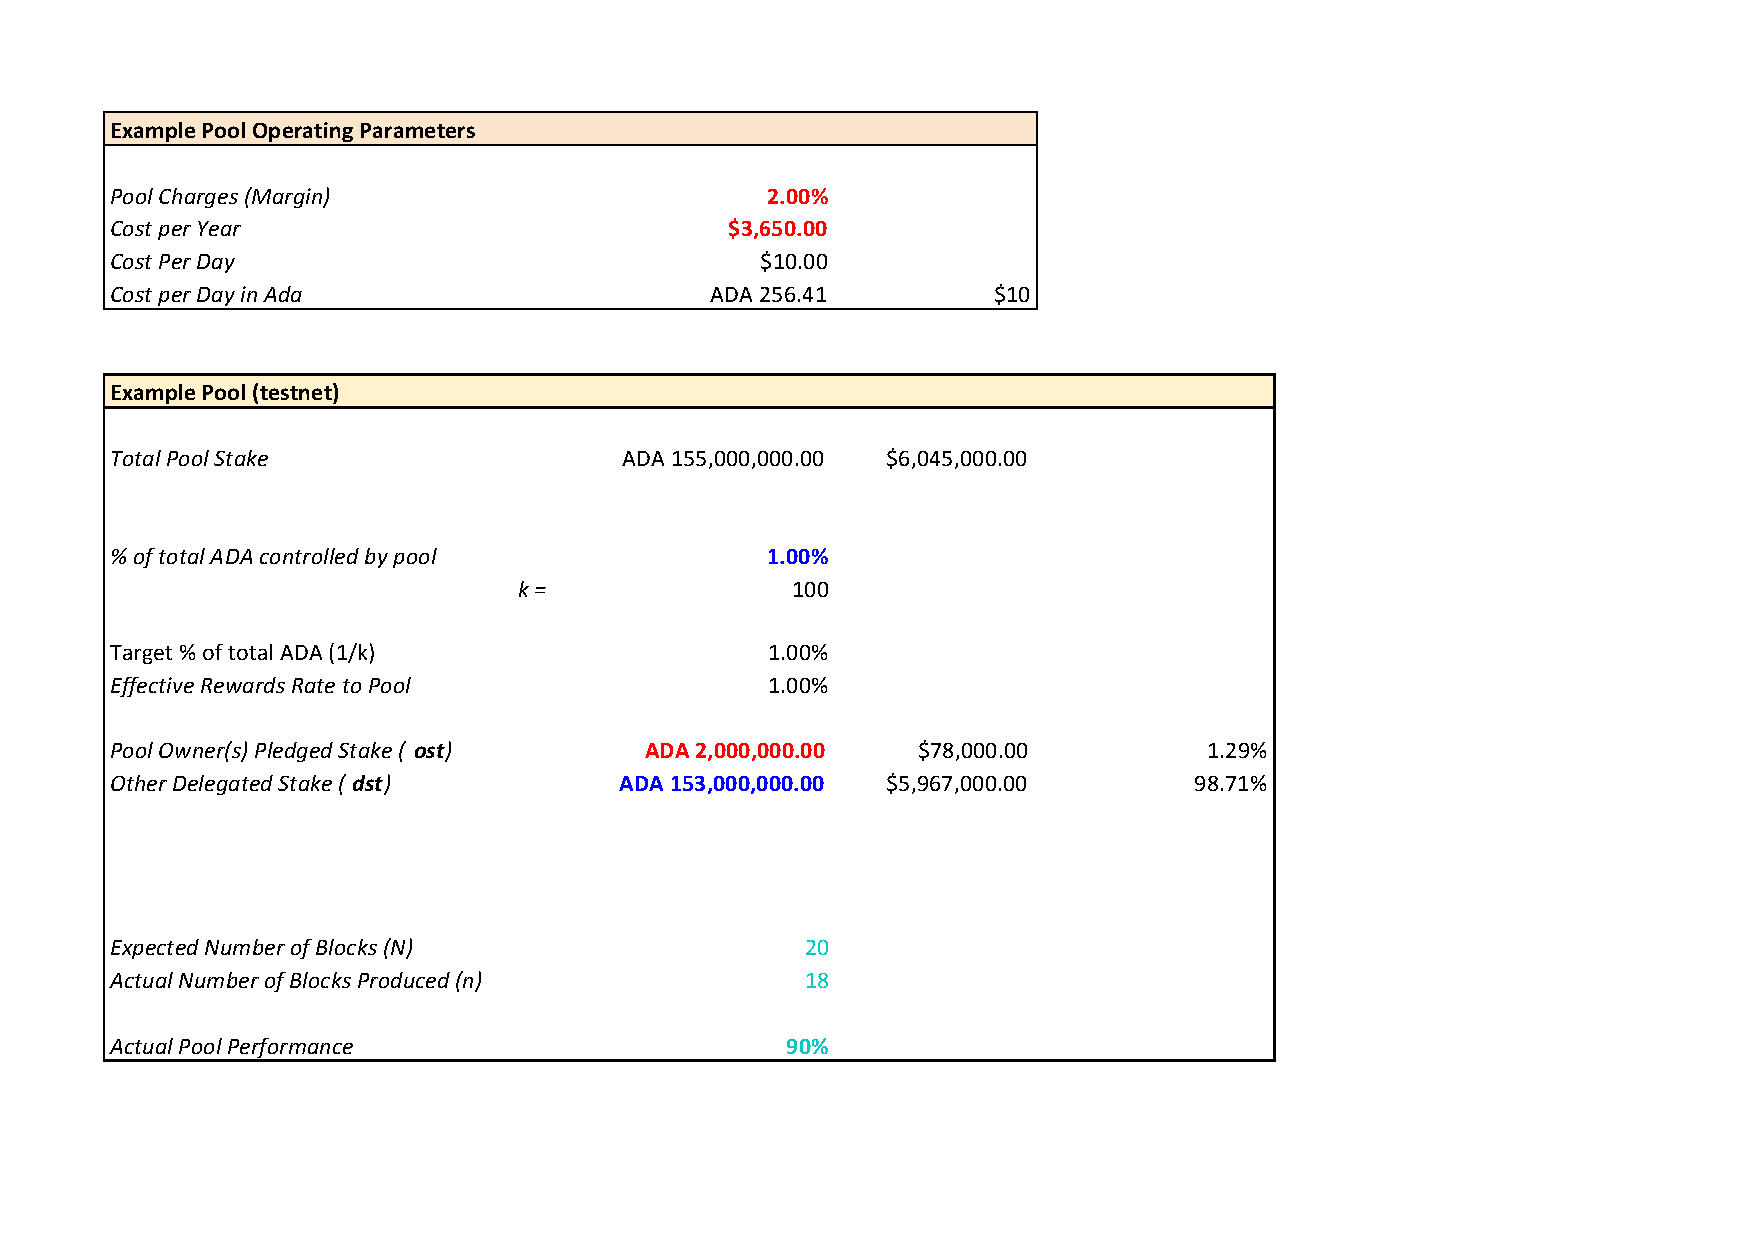
\includegraphics[width=1.2\textwidth]{RCT3.pdf}
\vspace{-0.5in}

\noindent
This diagram shows the StakePool-specific parameters, including the total controlled \ada{} and the
division by owner(s) and delegators.  Here, 98.71\% of the StakePool \ada{} is owned
by delegators.  We choose a \emph{margin} for the pool charges of 2.00\% of the net income,
and a daily \emph{cost} of \ADA{256.41} (\$10).
The gross reward to the StakePool is precisely the expected reward, since it controls
exactly the required percentage of stake (1.00\%, corresponding to the limit set from
the $k$ parameter).  This is reduced in line with the StakePool's \emph{actual performance}
as observed by the system (here assumed to be 90\%), giving a \emph{penalty} that amounts
to \ADA{3452.05} per day.

\clearpage
\subsubsection*{Calculated Rewards}

\hspace{-0.65in}\begin{minipage}{\textwidth}
%\vspace{-1in}
  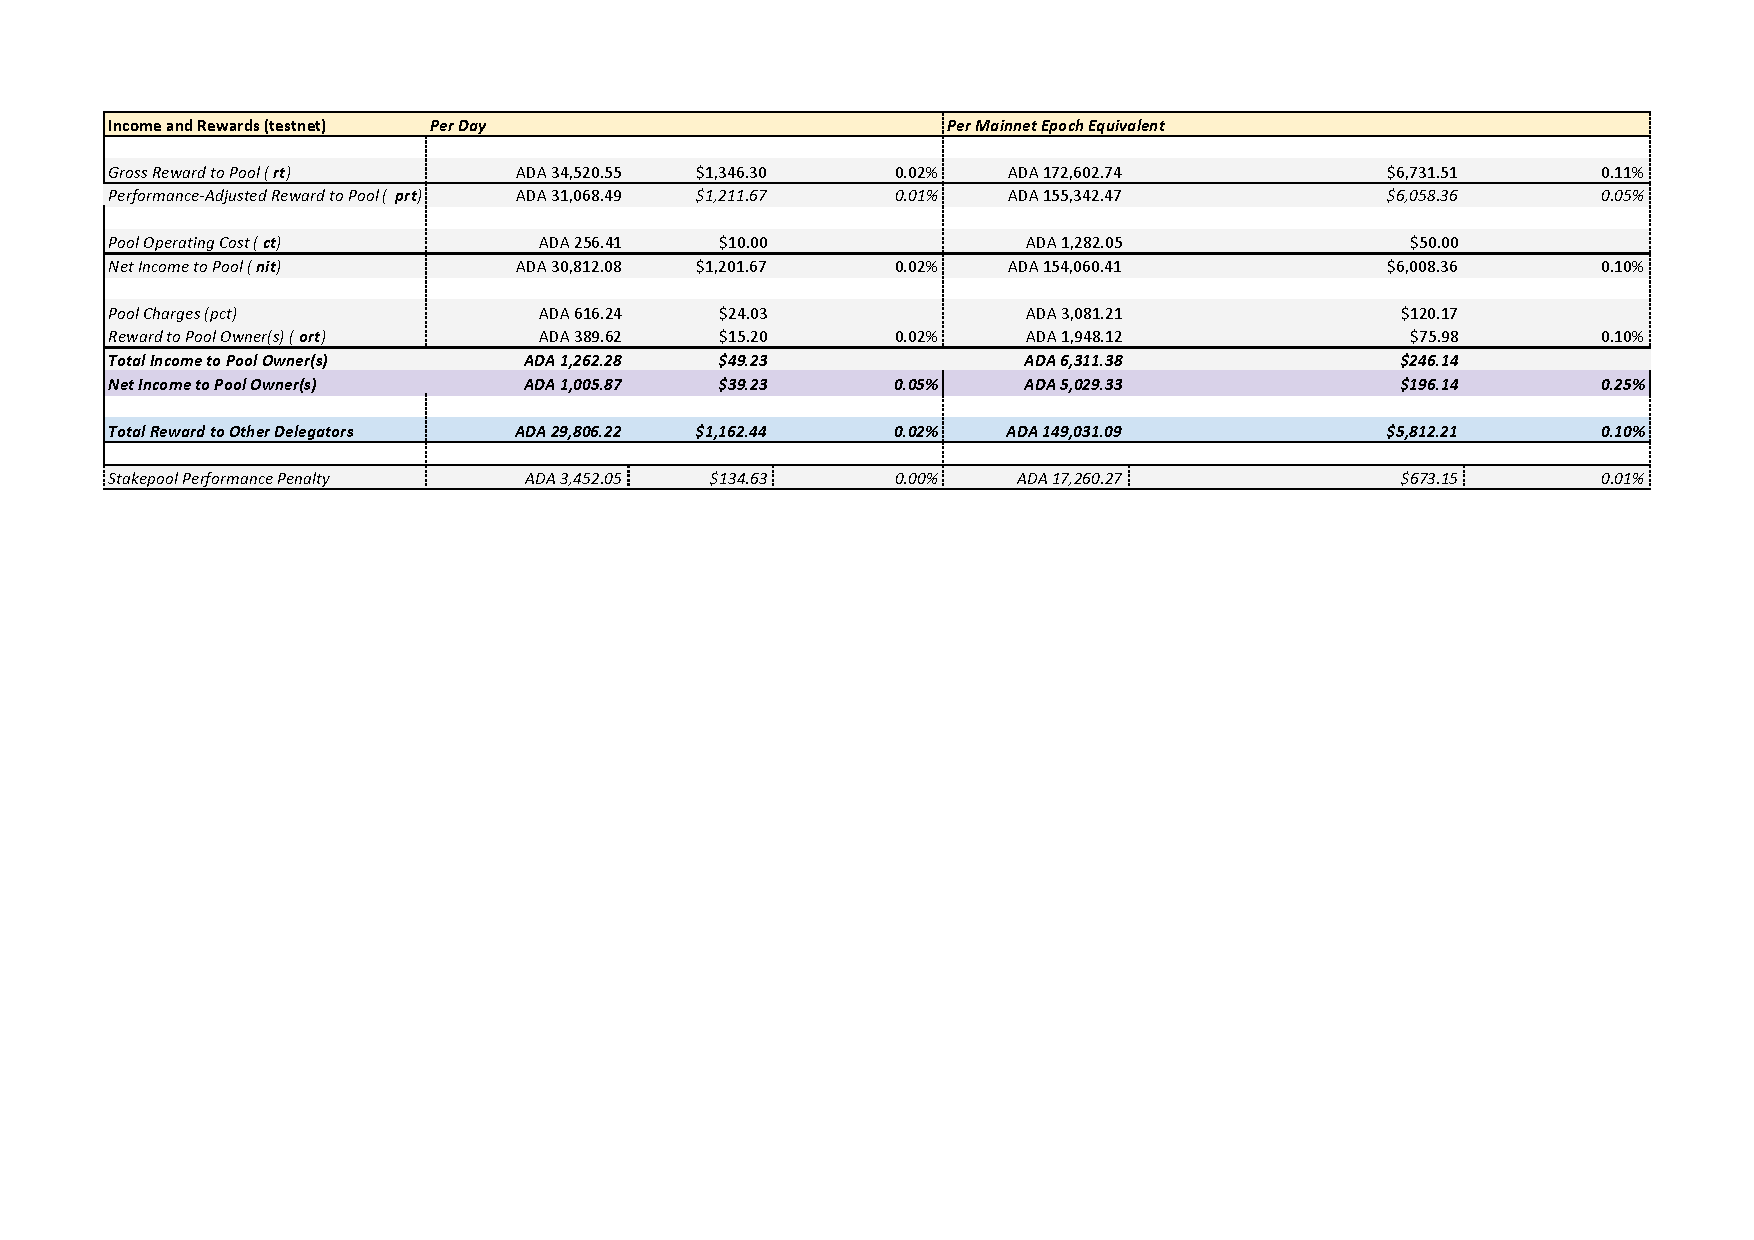
\includegraphics[width=1.2\textwidth]{RCT4.pdf}
\vspace{-3.8in}

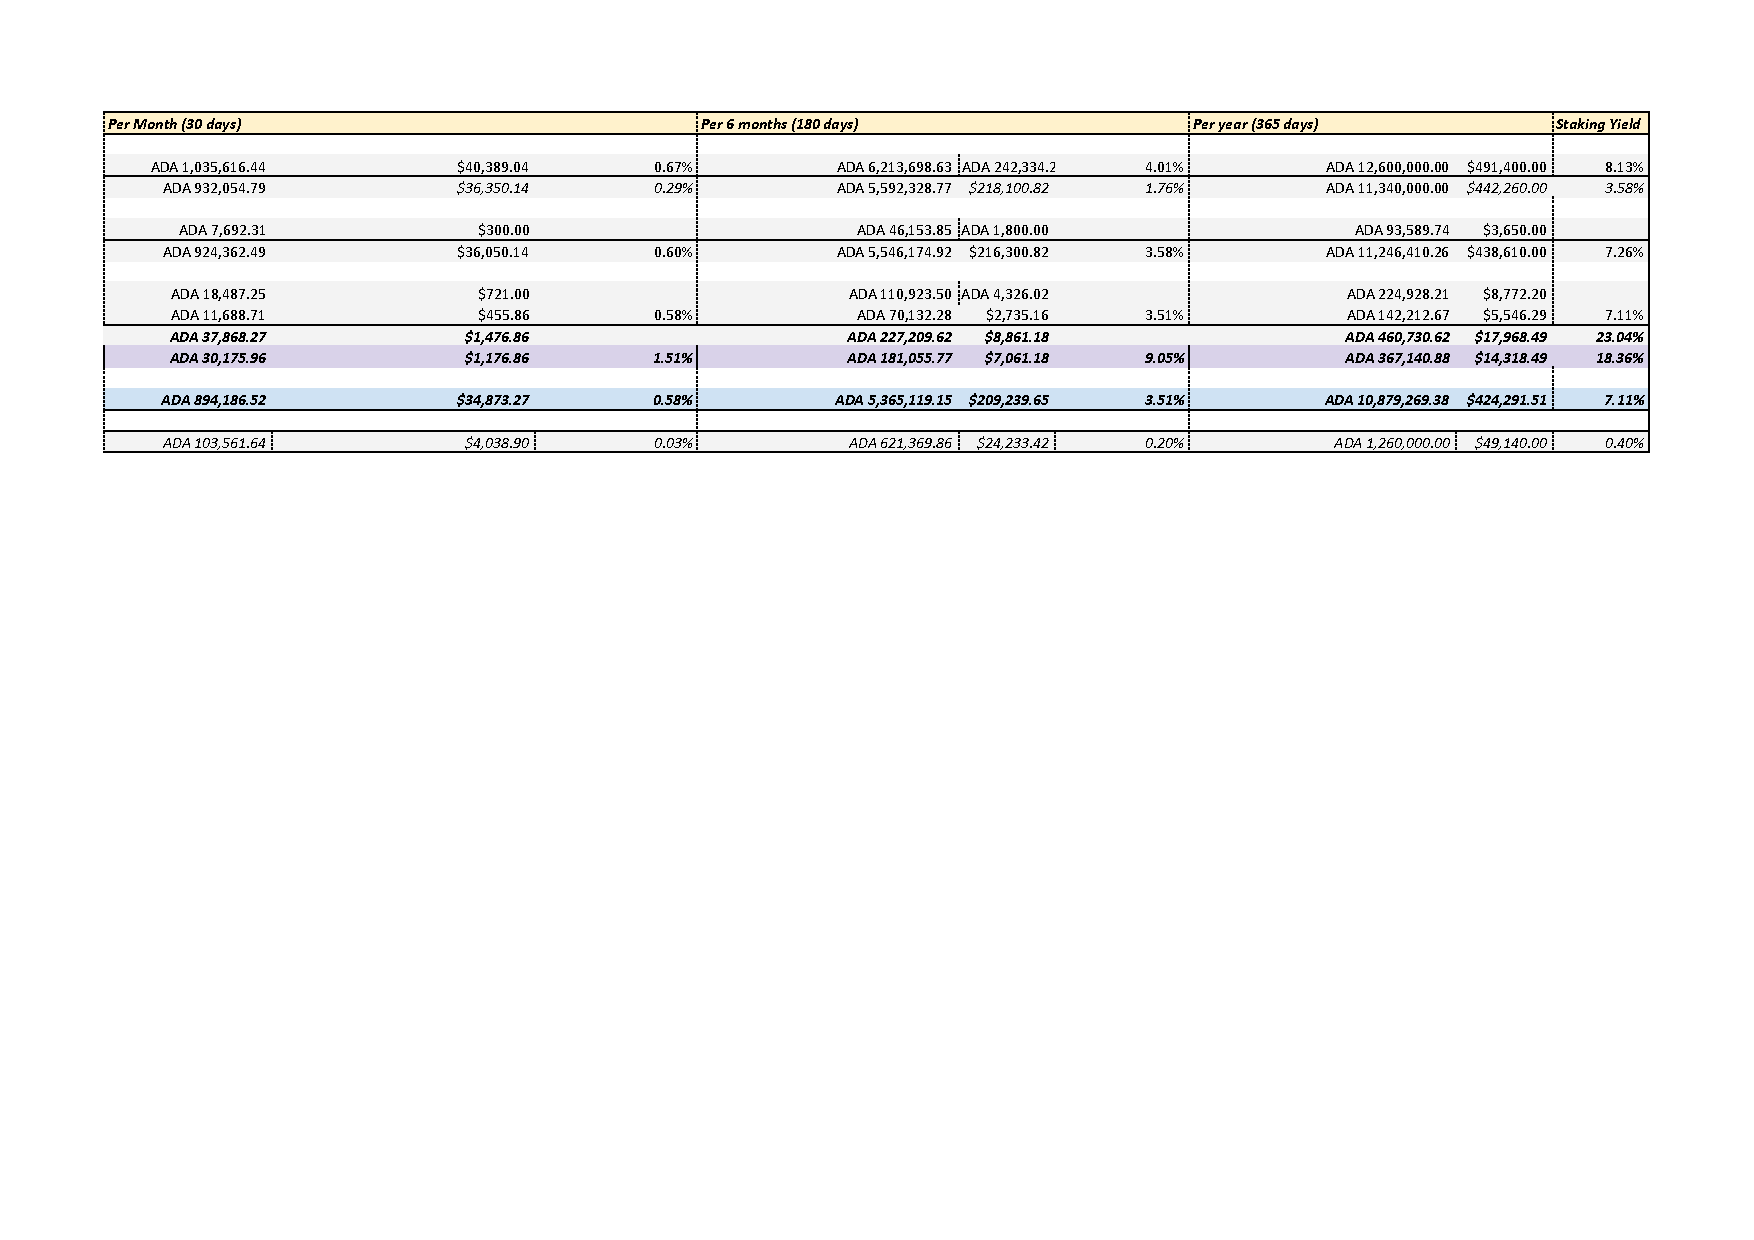
\includegraphics[width=1.2\textwidth]{RCT5.pdf}
\vspace{-3in}
\end{minipage}

\noindent
This diagram shows the corresponding rewards that accrue to the owner(s) and delegators,
plus a calculation of the total income that is received by the owners.  We will assume that the average
and actual gross rewards are the same, i.e. if the StakePool controls 1\% of the total \ada{} in
circulation, it will produce exactly 1\% of the blocks, that it has 100\% performance, and will therefore receive exactly 1\% of the rewards.
In total, the
owners and delegators to this StakePool would receive a net reward that was equivalent to 7.11\% per year
(the ``staking yield'').  If there were 4 owners for the StakePool, each would receive
25\% of the operator rewards, i.e. $\ADA{158,121.42} \div 4 ~~=~~ \ADA{39,530.355}$.
Similarly, a delegator contributing 10\% of the delegated stake would receive 10\% of
the delegator reward, i.e., $\ADA{12,096,288.83} \div 10 ~~=~~ \ADA{1,209,628.8883}$.


\subsection{How rewards are returned to Owners and Delegators}
\label{sec:rewards-return}

Rewards are returned through transactions using the relevant public keys, following the end
of each epoch (settlement may not be immediate, since the rewards may need to be audited, for example).
These rewards can then be stored within a wallet, recorded on an exchange etc., as required.
In the Incentivised TestNet, however, they cannot be used for further staking.
\khcomment{JC/MG to expand}

\clearpage
\section{The Full Incentives  Scheme (Shelley MainNet Implementation)}
\label{sec:MainNet}

The full incentives scheme that  be used in the MainNet adds several additional aspects to the
simple scheme above:

\begin{enumerate}
\item
  Transaction fees that are distributed to the StakePools;
\item
  StakePool deposits, part of which are added to the rewards;
\item
  An ``influence factor'', that determines how much influence the owner(s)' stake has on
  the desirability of a StakePool;
\item
  A monetary expansion rate that varies over time (decreasing in an exponential way);
\item
  The performance of the system as a whole is taken into account;
\item
  The apparent performance of the StakePool.
\end{enumerate}

\noindent
In addition, the number of days per epoch will be changed.  Collectively, these changes implement the \emph{non-myopic rewards} scheme of~\cite{delegation_design}.

\begin{figure}[h!]
\begin{center}
\begin{tabular}{||l|p{13cm}||}
  \hline \hline
  \textbf{Parameter} & \textbf{Definition} \\\hline
\textbf{\color{green}  $\textit{inf}$} & \textbf{\color{green} The influence Factor. The influence that the owner(s)' stake has on the
  desirability of a pool. This is a finite positive number, with 0 being no influence, and larger numbers being more influence. } \\\hline
\textbf{\color{cyan}  $\textit{Perf}_E$} & \textbf{\color{cyan} The ratio of the number of blocks that were actually produced in Epoch $E$ to the expected average number of blocks that should be produced in an Epoch.
  This will be derived from the number of slots in the Epoch.} \\\hline
\textbf{\color{cyan}$\textit{Fees}_E$} & \textbf{\color{cyan}All the transaction fees for Epoch $E$} \\\hline
\textbf{\color{cyan}$\textit{Deposits}_E$} & \textbf{\color{cyan} The non-refundable deposits for Epoch $E$} \\\hline
\textbf{\color{cyan} $\textit{MER}_E$} & \textbf{\color{cyan} The ``Monetary Expansion Rate'' for Epoch $E$}. \newline \textbf{\color{cyan} \emph{See Section~\ref{sec:expansion}.}} \\\hline
\hline
\end{tabular}
\end{center}
\caption{New Parameters used in the MainNet Incentives Calculation.}
\end{figure}

\clearpage
\begin{figure}[h!]
\begin{center}
\begin{tabular}{||l|l|p{6cm}|l||}
  \hline \hline
\textbf{Parameter} & \textbf{Expected Value} & \textbf{Description} & \textbf{Calculated as} \\\hline
%$E^{\textit{Test}}$ & 90-180 & Number of Epochs that the Incentivised TestNet persists & \\\hline
${\textit{Distr}}^{Test}$ & & The total Distribution of \ada{} that will be made by the Incentivised TestNet & \\\hline
$\textit{Ada}^{\textit{Circ}}_{0}$ & \ADA{31-31.5bn} & The \ada{} that is initially circulating in the MainNet & $\textit{Ada}^{\textit{Circ}}_{\textit{Test}} + {\textit{Distr}}^{\textit{Test}}$ \\\hline
$\textit{Ada}^{\textit{Rsv}}_{0}$ & \ADA{14-14.5bn} & The total \ada{} in the reserves at Shelley MainNet launch & $\textit{Ada}^{Tot} - \textit{Ada}^{\textit{Circ}}_{0}$ \\\hline
\hline
\end{tabular}
\end{center}
\caption{The \ada{} that is Initially in Circulation in the MainNet.}
\end{figure}

\noindent
The total \ada{} that will initially circulate in the MainNet, that is the \ada{} in circulation in Epoch 0 of the MainNet,
$\textit{Ada}^{\textit{Circ}}_{0}$ will be the \ada{} that was in circulation at the launch of the Incentivised
TestNet plus the total distribution that was made over the period of operation of the TestNet.
Since an equal amount of \ada{} is distributed per epoch in
the TestNet,
the distribution is will just be the multiple of the number of epochs that the Incentivised TestNet has
been active and the rewards distribution that has been made in each epoch.


\begin{figure}[h!]
\begin{center}
\begin{tabular}{||l|p{2.4cm}|p{6cm}|p{3.9cm}||}
  \hline \hline
\textbf{Parameter} & \textbf{Expected Initial Value} & \textbf{Description} & \textbf{Calculated as} \\\hline
$\textit{E}$ & $0$ & The Current MainNet Epoch, $0 \le E \le \infty$ & \\\hline
\textbf{\color{green} $\textit{DPE}$} & \textbf{\color{green} 5} & \textbf{\color{green} Days per Epoch: Duration of a \cardano{} Epoch} & \\\hline
\textbf{\color{cyan} $\textit{Fees}_E$} & & \textbf{\color{cyan} All the transaction fees for Epoch $E$} & \\\hline
\textbf{\color{cyan} $\textit{Deposits}_E$} & & \textbf{\color{cyan} The non-refundable deposits for Epoch $E$} & \\\hline
$\textit{MER}_E$ & 10\%-15\% &  The ``Monetary Expansion Rate'' for Epoch $E$ & \emph{See Section~\ref{sec:expansion}.} \\\hline
$\textit{Perf}_E$ & 80\%-100\% &  The Overall Performance of the MainNet in Epoch $E$ &  \\\hline
$\textit{Distr}_E$ & approx. \ADA{62M} & Gross Distribution for Epoch $E$ & \begin{flushleft}$\textit{Ada}^{\textit{Rsv}}_E \times \textit{MER}_E \times \textrm{min}(\textit{Perf}_E, 100\%)$ \end{flushleft} \\\hline
$\textit{Ada}^{\textit{Circ}}_E$ & approx. \ADA{31.5bn}  & \ada{} in circulation in Epoch $E$ & $\textit{Ada}^{\textit{Circ}}_{E-1} + \textit{Distr}_E$ \\\hline
$\textit{Ada}^{\textit{Rsv}}_E$ & approx. \ADA{14.5bn} & \ada{} in reserve in Epoch $E$ & $\textit{Ada}^{\textit{Rsv}}_{E-1} - \textit{Distr}_E$ \\\hline
$R_E$ & approx. \ADA{56M} & Total Rewards per Epoch & $ (\textit{Distr}_E + \textit{Fees}_E + \textit{Deposits}_E) \div (\textit{inf}+1)$ \\\hline
% $T_E$ & approx. \ADA{5.6M} & Treasury Top Slice for Epoch $E$ & $R_E \times T$ \\\hline
  \hline
\end{tabular}
\end{center}
\caption{Total Distribution and Rewards per Epoch in the MainNet, with expected values for the first MainNet Epoch (Epoch 0).}
\end{figure}

\noindent
In the MainNet, the gross rewards distribution will depend on the current MainNet Epoch, $E$, and will reduce over time.
The total \ada{} that is distributed during epoch $E$ in the MainNet (${\textit{Distr}}_E$) is calculated from the current
value of the \ada{} reserves, $\textit{Ada}^{\textit{Rsv}}_E$, and the variable \emph{monetary expansion rate} that is in force for
the current epoch, $\textit{MER}_E$.
%
This distribution is restricted by the \emph{overall performance}, $\textit{Perf}_E$, which is defined as a fraction of the \emph{expected performance} during Epoch $E$.
%
The reserves will be depleted by the amount of new \ada{} that is distributed in the Epoch, $\textit{Distr}_E$. This gives the
value of the reserve for the next Epoch, $\textit{Ada}^{\textit{Rsv}}_{E+1}$.  The \ada{} in circulation, $\textit{Ada}^{\textit{Circ}}_{E+1}$
is correspondingly increased by the amount that has been distributed.
%
Fees and non-returned deposits are added to the reward distribution.  This total distribution is then modified by the \emph{influence factor}
(the higher the influence factor, the lower the total rewards) to give the total rewards per epoch, $R_E$.

% \khcomment{Check when: before/after reserves.}  Checked.
%
% As before, the top slice that is allocated to the treasury ($T_E$) is
% deducted from this distribution, and the remainder is then allocated to the StakePools as rewards ($R_E$).

\subsection{The Monetary Expansion Rate}
\label{sec:expansion}

\begin{figure}[h!]
  \begin{center}
    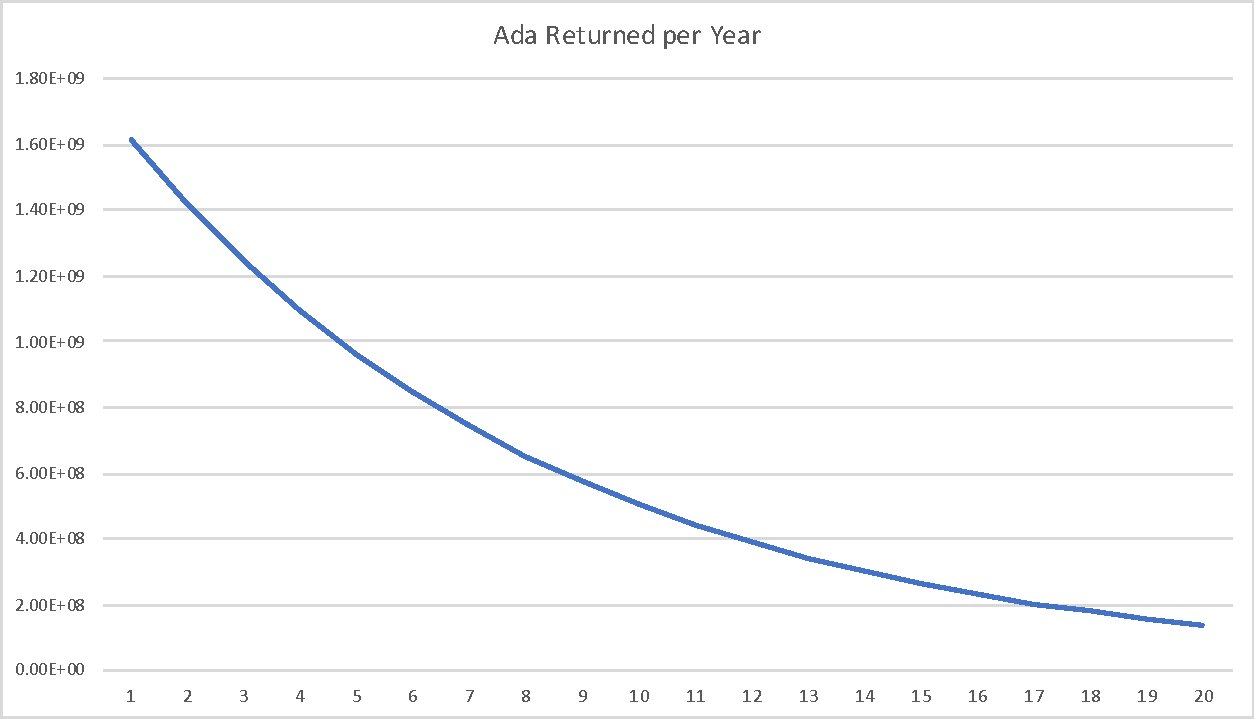
\includegraphics[width=0.75\textwidth]{AdaPerYear.pdf}
\\[2ex]
    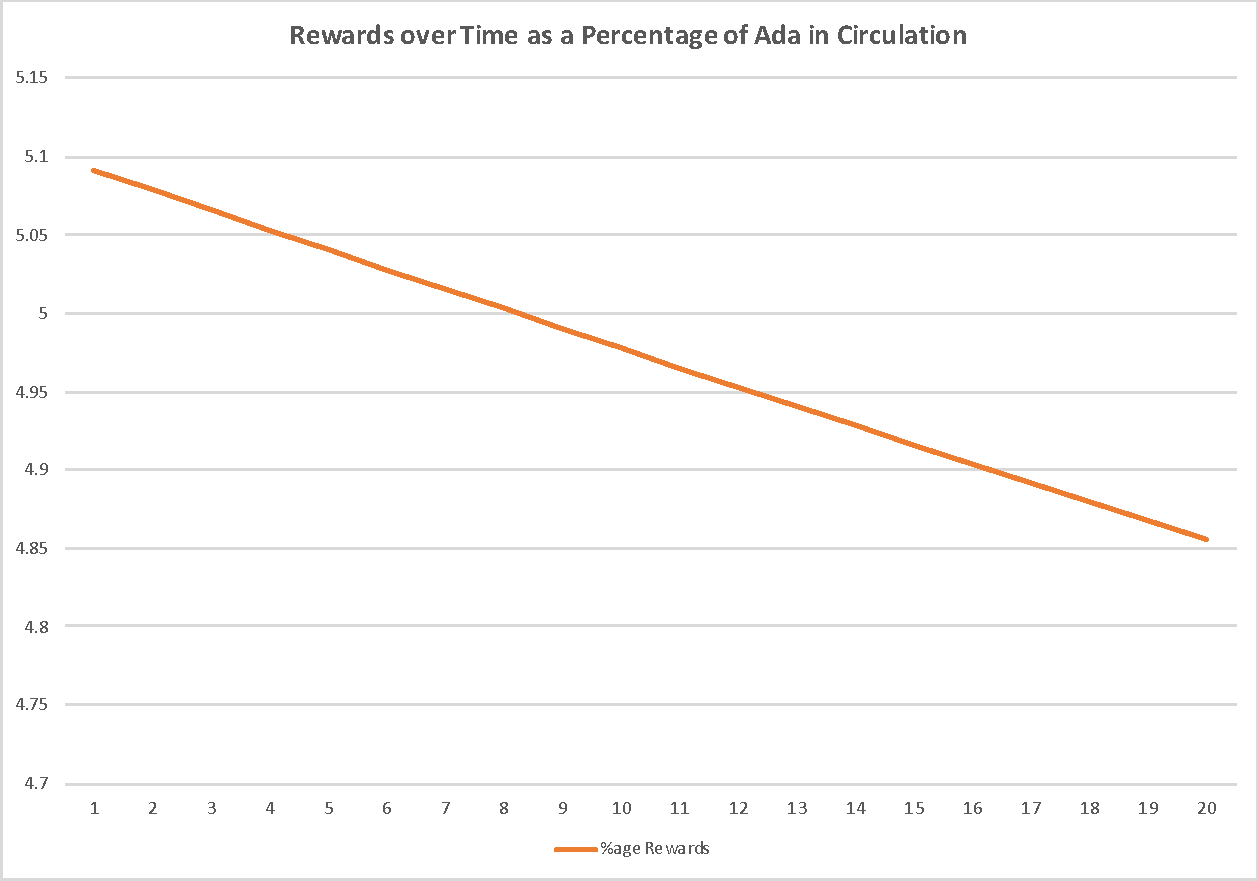
\includegraphics[width=0.75\textwidth]{Rewards.pdf}
  \end{center}
  \caption{Ada Rewards over Time, assuming $R^{\textit{Avg}}$=0.05, $\textit{Fee}_E$=2000, $\textit{Perf}_E=100\%$.}
\end{figure}

\noindent
The monetary expansion rate for Epoch $E$ is determined by the following equation:

$$
\textit{MER}_E ~~=~~ \frac{\textit{Ada}^{Circ}_E \times (\sqrt[\textit{EPY}]{1+R^{\textit{Avg}}} - 1) - (1- T) \times \textit{Fees}_E}
                          {(1-T) \times \textit{min}(\textit{Perf}_E,100\%) \times (\textit{Ada}^{Tot} - Ada^{Circ}_E)}
$$

\noindent
where $R^{\textit{Avg}}$ is the expected average rewards per \ada{} per year, and $\textit{EPY}$ is the number of epochs per year (73 in non-leap years if
$\textit{DPE} = 5$). $T$ is the pre-defined Treasury Top Slice (initially 10\%).
%
Assuming $R^{\textit{Avg}}$=0.05, $\textit{Fee}_E$=2000, and $\textit{Perf}_E=99\%$, with the other values as above, then we obtain
$\textit{MER}_0 = 0.00178650067$, equating to monetary expansion of 13.04\% over a year.

\subsection{Transaction Fees}
\label{sec:fees}

The fee for each transaction $t$ is calculated as follows:

$$
\textit{Fee} (t) ~=~ a + b \times \textit{size}(t)
$$

\noindent
where $a$ is a fixed fee for each transaction, and $b$ calculates an additional fee from the transaction size ($\textit{size}(t)$).

\clearpage
\subsection{The Rewards that are received by a StakePool for Epoch $E$}

\begin{figure}[h!]
\begin{center}
\begin{tabular}{||l|l|p{6cm}|l||}
  \hline \hline
\textbf{Parameter} & \textbf{Expected Value} & \textbf{Definition} & \textbf{Calculated as} \\\hline
\textbf{\color{red} $\textit{\textit{Pool}}^{\textit{Cost}}$} &  & \textbf{\color{red} Cost per day in \ada{}} & \\\hline
\textbf{\color{red} ${\textit{Pool}}^{\textit{Margin}}$} &  \textbf{\color{red} 0\%-100\%} & \textbf{\color{red} Percentage fee on rewards (the ``margin'')} & \\\hline
\textbf{\color{red} ${Pool}^\textit{Pledge}$} & & \textbf{\color{red} \ada{} that is pledged to the StakePool by the Owner(s)} & \\\hline
\textbf{\color{blue} ${\textit{Pool}}^\textit{Deleg}$} & & \textbf{\color{blue} \ada{} that is delegated to the StakePool} & \\\hline
${\textit{Pool}}^{Tot}$ & & All \ada{} that is controlled by the StakePool & ${\textit{Pool}}^\textit{Pledge} + {\textit{Pool}}^\textit{Deleg}$ \\\hline
${\textit{Pool}}^\%$ & & Fraction of the \ada{} in circulation that is controlled by the StakePool & {\large $\frac{{\textit{Pool}}^{Tot}}{\textit{Ada}^{\textit{Circ}}_E}$} \\\hline
${\textit{Pledge}}^\%$ & & Fraction of the \ada{} in circulation that is \emph{pledged} to the StakePool by the Owner(s) & {\large $\frac{{\textit{Pool}}^{Pledge}}{\textit{Ada}^{\textit{Circ}}_E}$} \\\hline
&&&  \\\hline
\textbf{\color{green} \emph{k}} & \textbf{\color{green} 50-1000} & \textbf{\color{green} The Target Number of StakePools} & \\\hline
\emph{z} & 0.001-0.02 & The Rewards Limit Fraction & $\frac{1}{k}$ \\\hline
%\emph{s'} & & The Effective Rewards Rate to Owner(s) & $\textrm{min} (s,z)$\\\hline
&&&  \\\hline
\textbf{\color{cyan} $\textit{Pool}^{\textit{Perf}}$} & & \textbf{\color{cyan} The \emph{Apparent Performance} of the StakePool} & \\\hline
  \hline
\end{tabular}
\end{center}
\caption{Parameters Governing the Rewards to a StakePool in a given Epoch, $E$.}
\label{fig:rewards-MainNet}
\end{figure}

\noindent
The parameters that govern the StakePool reward calculation are shown above.  Compared with the Incentivised
TestNet, the only new parameters are the effective rewards rate to the owner(s), $s'$, and the apparent performance of the StakePool, $\textit{Pool}^{\textit{Perf}}$.
The effective rewards rate limits the rewards that the owners can receive.  The \emph{apparent performance} of a StakePool is calculated
by dividing the fraction of blocks that the StakePool has created by the fraction of the total stake that it controls.  This may be more than 100\%.

\begin{figure}[h!]
\begin{center}
\begin{tabular}{||l|p{6cm}|l||}
  \hline \hline
  \textbf{Parameter}  & \textbf{Definition} & \textbf{Calculated as} \\\hline
  $s^\%$ & The \emph{effective} stake & $\textrm{min} (z,{\textit{Pool}}^\%)$ \\\hline
  $p^\%$ & The \emph{effective} pledge  & $\textrm{min} (z,{\textit{Pledge}}^\%) $ \\\hline
  $\textit{R}^\textit{Factor}$ & Overall StakePool rewards factor, taking into account the influence factor and rewards limit. & $s^\% \times \textit{inf} \times ((s^\% - p^\% \times (z - s^\%)) \div z)$ \\\hline
  $R^{Optimal}$ & The Optimal Gross Reward to the StakePool.  \textbf{This will be reduced to 0 if any Owner(s)' \emph{pledge} is not honoured.} & $R_E \times \textit{R}^{Factor}$ \\\hline
$R^{\textit{Gross}}$ & The Actual Gross Reward to the StakePool & $R^{Optimal} \times \textit{Pool}^{\textit{Perf}}$ \\\hline
%${\textit{Pool}}^{\textit{Fees}}$ & The fees the StakePool earns from each transaction & \\\hline
${\textit{Pool}}^{\textit{Cost}}_E$ & Pool Operator Costs for the Epoch & $\textrm{min}(\textit{\textit{Pool}}^{\textit{Cost}} \times \textit{DPE},R^{\textit{Gross}})$ \\\hline
$R^{\textit{Net}}$  & The Net Reward to the StakePool & $R^{\textit{Gross}} - {\textit{Pool}}^{\textit{Cost}}_E$ \\\hline
$R^{\textit{Owner}}$ & The Total Reward to the Owner(s) & $R^{\textit{Net}} \times {\textit{Pool}}^{\textit{Margin}} $ \\\hline
$R^{\textit{Deleg}}$ & The Total Reward to the Delegators & $R^{\textit{Net}} \times (100\% - {\textit{Pool}}^{\textit{Margin}})$ \\\hline
$\textit{Owner}^\textit{Income}$ & The Total Pool Owner Income & ${\textit{Pool}}^{\textit{Cost}}_E + R^{Owner}$ \\\hline
\hline
\end{tabular}
\end{center}
\caption{Calculation of the Total Stake Pool Reward.}
\end{figure}

\noindent
As before, the gross reward that is received by the StakePool is, on average, directly proportional to the
stake that it controls, as a proportion of the total \ada{} that is in circulation.
The \emph{optimal} reward is limited by the pre-calculated \emph{rewards limit fraction}, and is further reduced in
proportion to its \emph{apparent performance}, $\textit{Pool}^{\textit{Perf}}$.
The fees are added to this sum.
Once the pool operator costs are subtracted,
the net reward is then distributed to the owner(s) and delegators.
The delegator reward is calculated as in the Incentivised TestNet, in proportion to the stake that has
been delegated to the StakePool.
The owner(s) reward is, however, limited by $p^\%$, the \emph{effective rewards rate} to the owner(s).
%
The StakePool owner income is then the sum of the operator costs and the pool owner rewards.
\textbf{Note that, as before, if there is insufficient gross reward to cover the operator costs, all the reward will be used to cover those
costs, leaving no further reward to be distributed to the either owners or delegators.
Note also that if any Owner withdraws their \emph{pledge} from the StakePool, no rewards will be received by the Owner(s) or the Delegator(s).}

\subsubsection*{The Rewards that are received by each Delegator for Epoch $E$}

\begin{figure}[h!]
\begin{center}
\begin{tabular}{||l|p{9cm}|l||}
  \hline \hline
\textbf{Parameter} & \textbf{Definition} & \textbf{Calculated as} \\\hline
${\textit{Pool}}^{Tot}$ & All \ada{} that is controlled by the StakePool & ${\textit{Pool}}^\textit{Pledge} + {\textit{Pool}}^\textit{Deleg}$ \\\hline
$R^{Deleg}$ & The Total Reward to the Delegators & $R^{\textit{Net}} - R^\textit{Owner}$ \\\hline
$D^{Stake}$ & The \ada{} that is delegated by Delegator $D$ & \\\hline
$D^\%$ & The proportion of \ada{} in the StakePool that is delegated by $D$ & $\frac{D^{Stake}}{Pool^{Tot}}$ \\\hline
$D^{Rewards}$ & The \ada{} rewards that are received by $D$ & $R^{\textit{Net}} \times D^\%$ \\\hline
\hline
\end{tabular}
\end{center}
\caption{The Rewards that are received by a specific Delegator, $D$.}
\end{figure}

\noindent
The rewards that are received by an individual delegator are calculated in exactly the same way as in
the Incentivised TestNet.  Each delegator receives rewards that are directly proportional to the
stake that that delegator has placed in the StakePool.  These are calculated from the net rewards to the
StakePool after deducting the owner rewards.

\clearpage
\subsubsection*{The Rewards that are received by each StakePool Owner for Epoch $E$}

% \khcomment{Check this, should be reduced by p^\%axxs.}  OK.

\begin{figure}[h!]
\begin{center}
\begin{tabular}{||l|p{9cm}|l||}
  \hline \hline
\textbf{Parameter}  & \textbf{Definition} & \textbf{Calculated as} \\\hline
$R^\textit{Owner}$ & The Total Reward to the Owner(s).  & $R^{\textit{Net}} \times {\textit{Pool}}^{\textit{Margin}}$ \\\hline
$O^\textit{Stake}$ & The \ada{} that is pledged by Owner $O$ & \\\hline
$O^\%$ & The proportion of \ada{} in the StakePool that is pledged by $O$ & $\frac{O^{Stake}}{Pool^{Tot}}$ \\\hline
$O^{Rewards}$ & The \ada{} rewards that are received by $O$. This may be capped if the owner fraction is too large,
as described in Section~\ref{sec:penalties}, or reduced to zero if any owner fails to honour their pledge. & $R^{\textit{Net}} \times O^\%$ \\\hline
\hline
\end{tabular}
\end{center}
\caption{The Rewards that are received by each Owner, $O$.}
\end{figure}

\noindent
In the MainNet, each owner receives rewards that are proportional to the stake that they have pledged,
calculated similarly to the delegator rewards.  If one or more StakePool owners withdraw their pledge during the epoch,
however, then no owner rewards will be received by any owner of that StakePool.


\clearpage
\subsection{The Rewards that are allocated to the Treasury for Epoch $E$}

In the MainNet, all rewards that are not allocated to StakePools will accrue to the treasury.  This will include some fraction of the
monetary expansion $\textit{MER}_E$, plus any penalties.  This will always be a positive value.

\subsubsection*{StakePool Rewards Penalties}
\label{sec:penalties}

Any rewards that are not allocated to a StakePool will accrue to the Treasury instead.  This can happen: % \khcomment{Check this.}

\begin{enumerate}[i)]
\item
  because of poor \emph{apparent performance}, $\textit{Pool}^{\textit{Perf}}$;
\item
  because one or more owners of a StakePool have failed to honour their \emph{pledge} (in which case \textbf{all} reward will accrue to the Treasury);
\item
  because the StakePool as a whole has exceeded the target size as governed by the $k$ and $z$ parameters;
\item
  because the Owner(s)' stake has exceeded the target size as governed by the $k$ and $z$ parameters.
\end{enumerate}

\noindent
Returning the rewards to the Treasury ensures that the \ada{} remains in circulation and can be re-allocated in future.
%, so providing a predictable rate
% of monetary expansion ($\textit{MER}_E$), as described in Section~\ref{sec:expansion}.



\subsection{Calculating Rewards in External Currencies}

Rewards can be converted to other currencies using the current exchange rate, exactly as described in
Section~\ref{sec:conversion}.  Realising these funds will require the use of an external \emph{exchange} service.

\clearpage
\subsection{Worked Example: Full Scheme}

This example is taken from the \IOHK{} internal calculator at
\url{https://docs.google.com/spreadsheets/d/1m_CfNMdkxR_OrfRwThbU-6faxHUf7NdIhDLc6r-4lIM/edit#gid=1365573139}.

\subsubsection*{Key Parameters}

\hspace{-0.65in}\begin{minipage}{\textwidth}
\noindent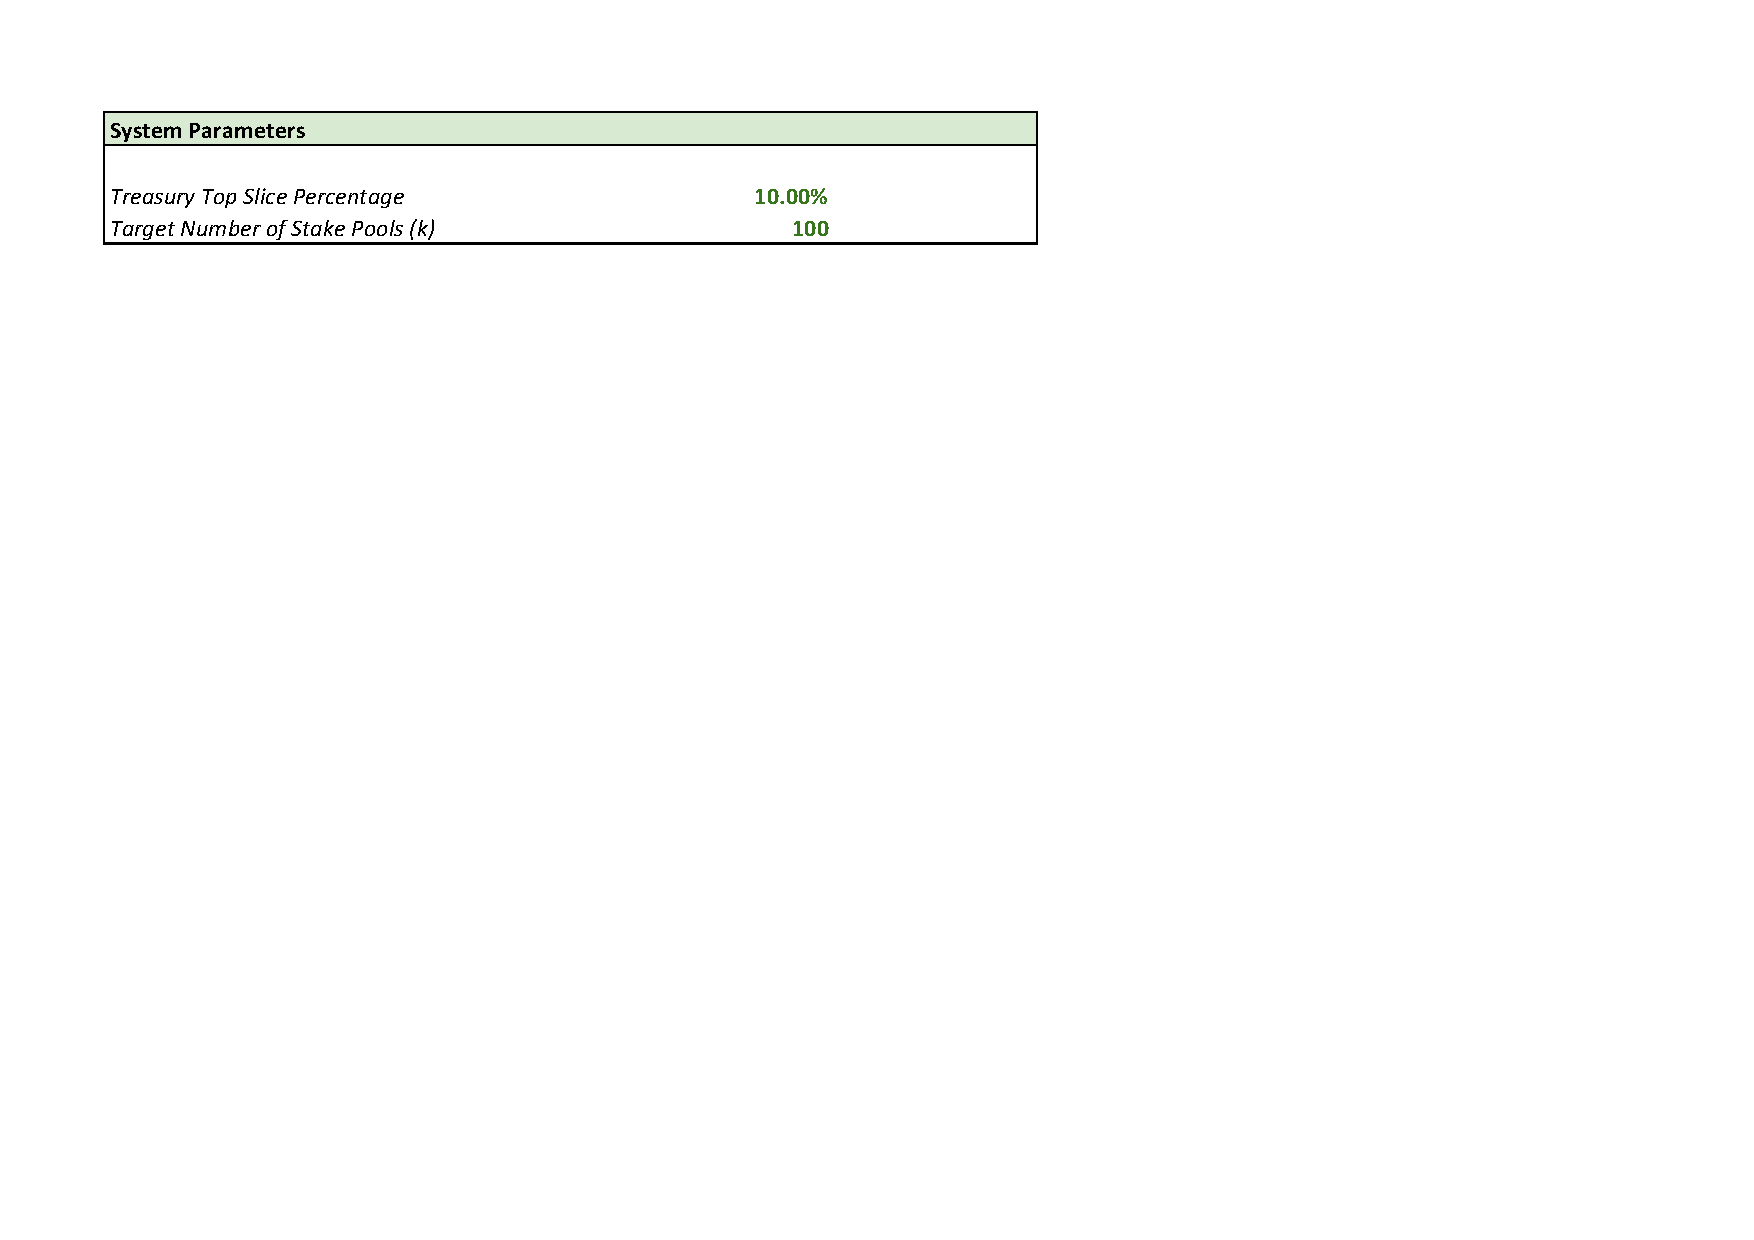
\includegraphics{RCM0.pdf}
\vspace{-7in}

\noindent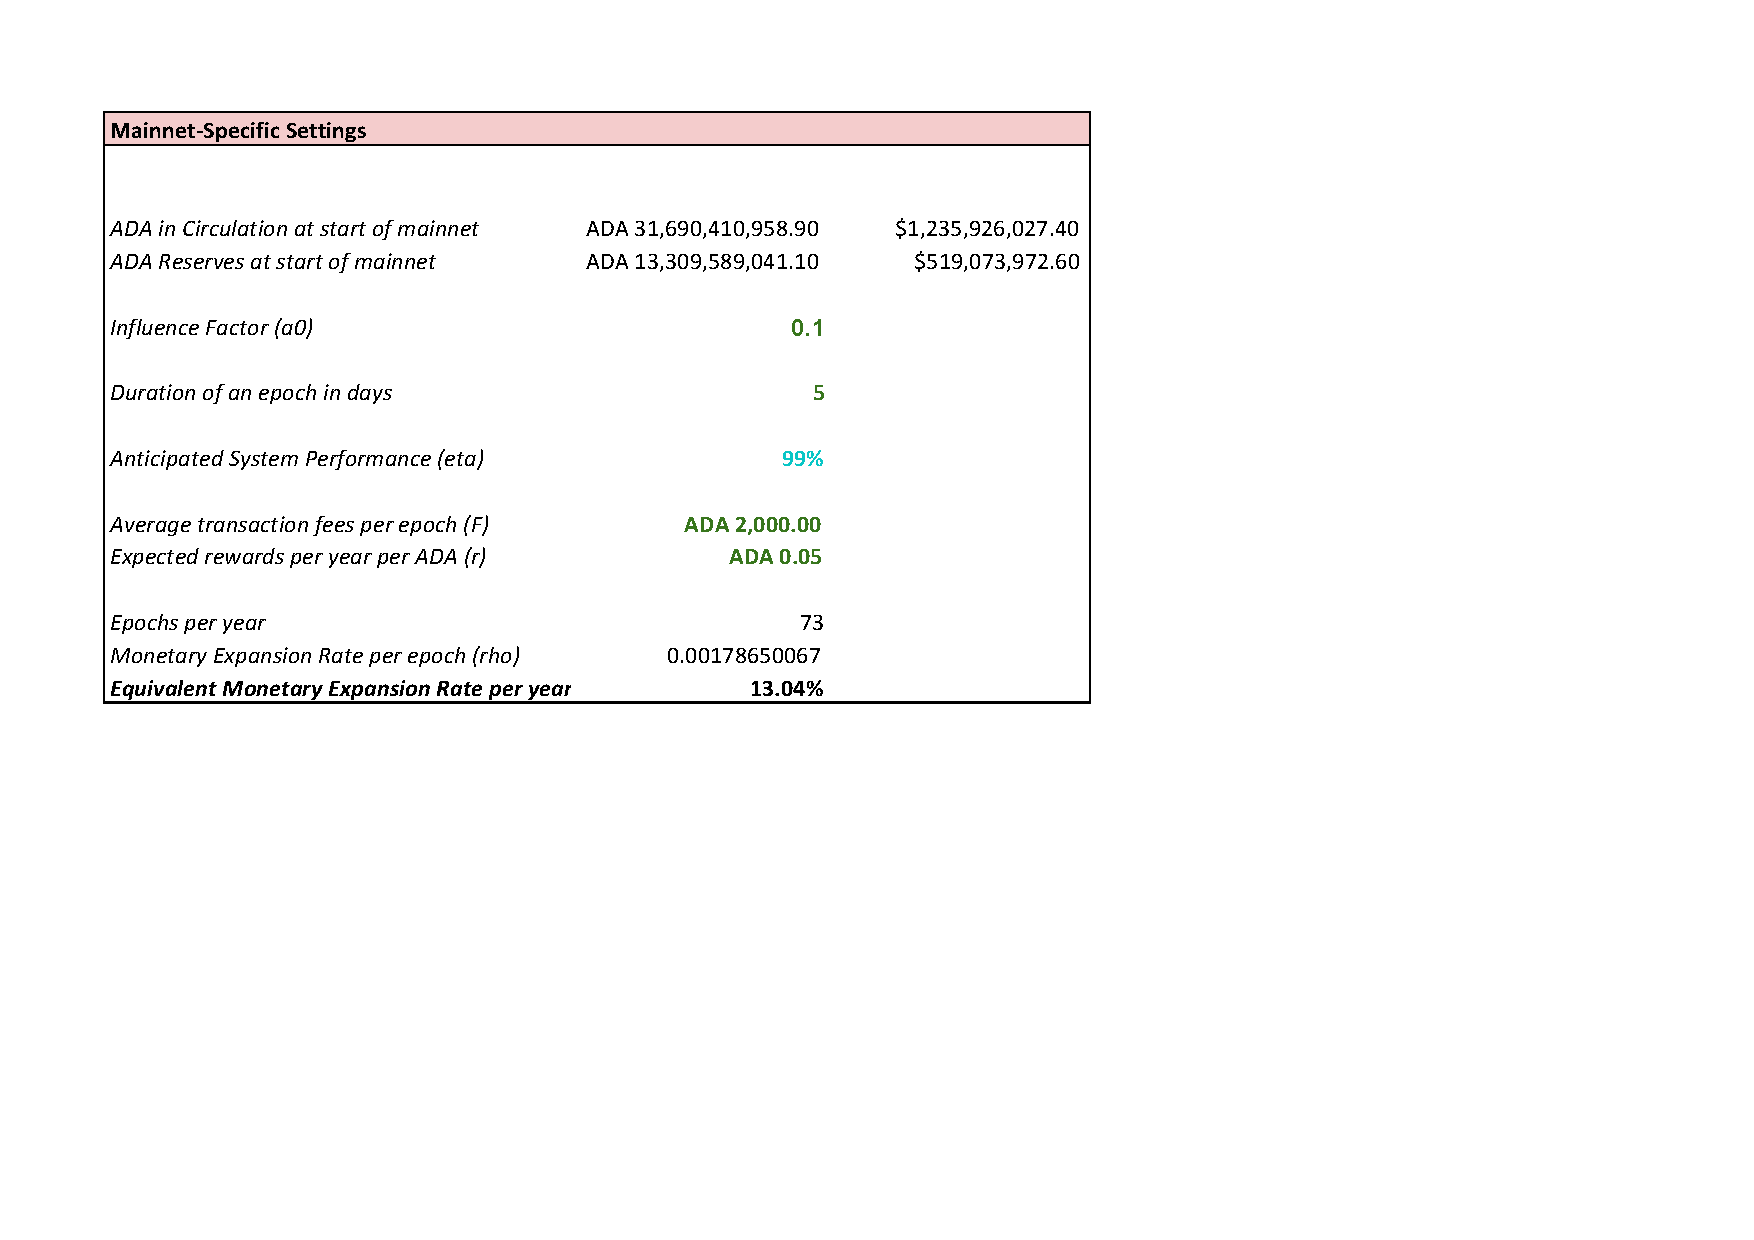
\includegraphics{RCM1.pdf}
\vspace{-3in}
\end{minipage}

\noindent
This diagram shows the key parameters and settings for the rewards system, including the initially
circulating and reserve \ada{}.  The monetary expansion rate is calculated as described above.
The number of days per Epoch is set to 5, the influence factor to 0.1, the system performance
to 99\%, the average transaction fees to \ADA{2,000} and the expected rewards rate to 0.05.
These parameters are used as part of the monetary expansion rate calculation.


\subsubsection*{Circulation and Distribution}

\hspace{-0.65in}
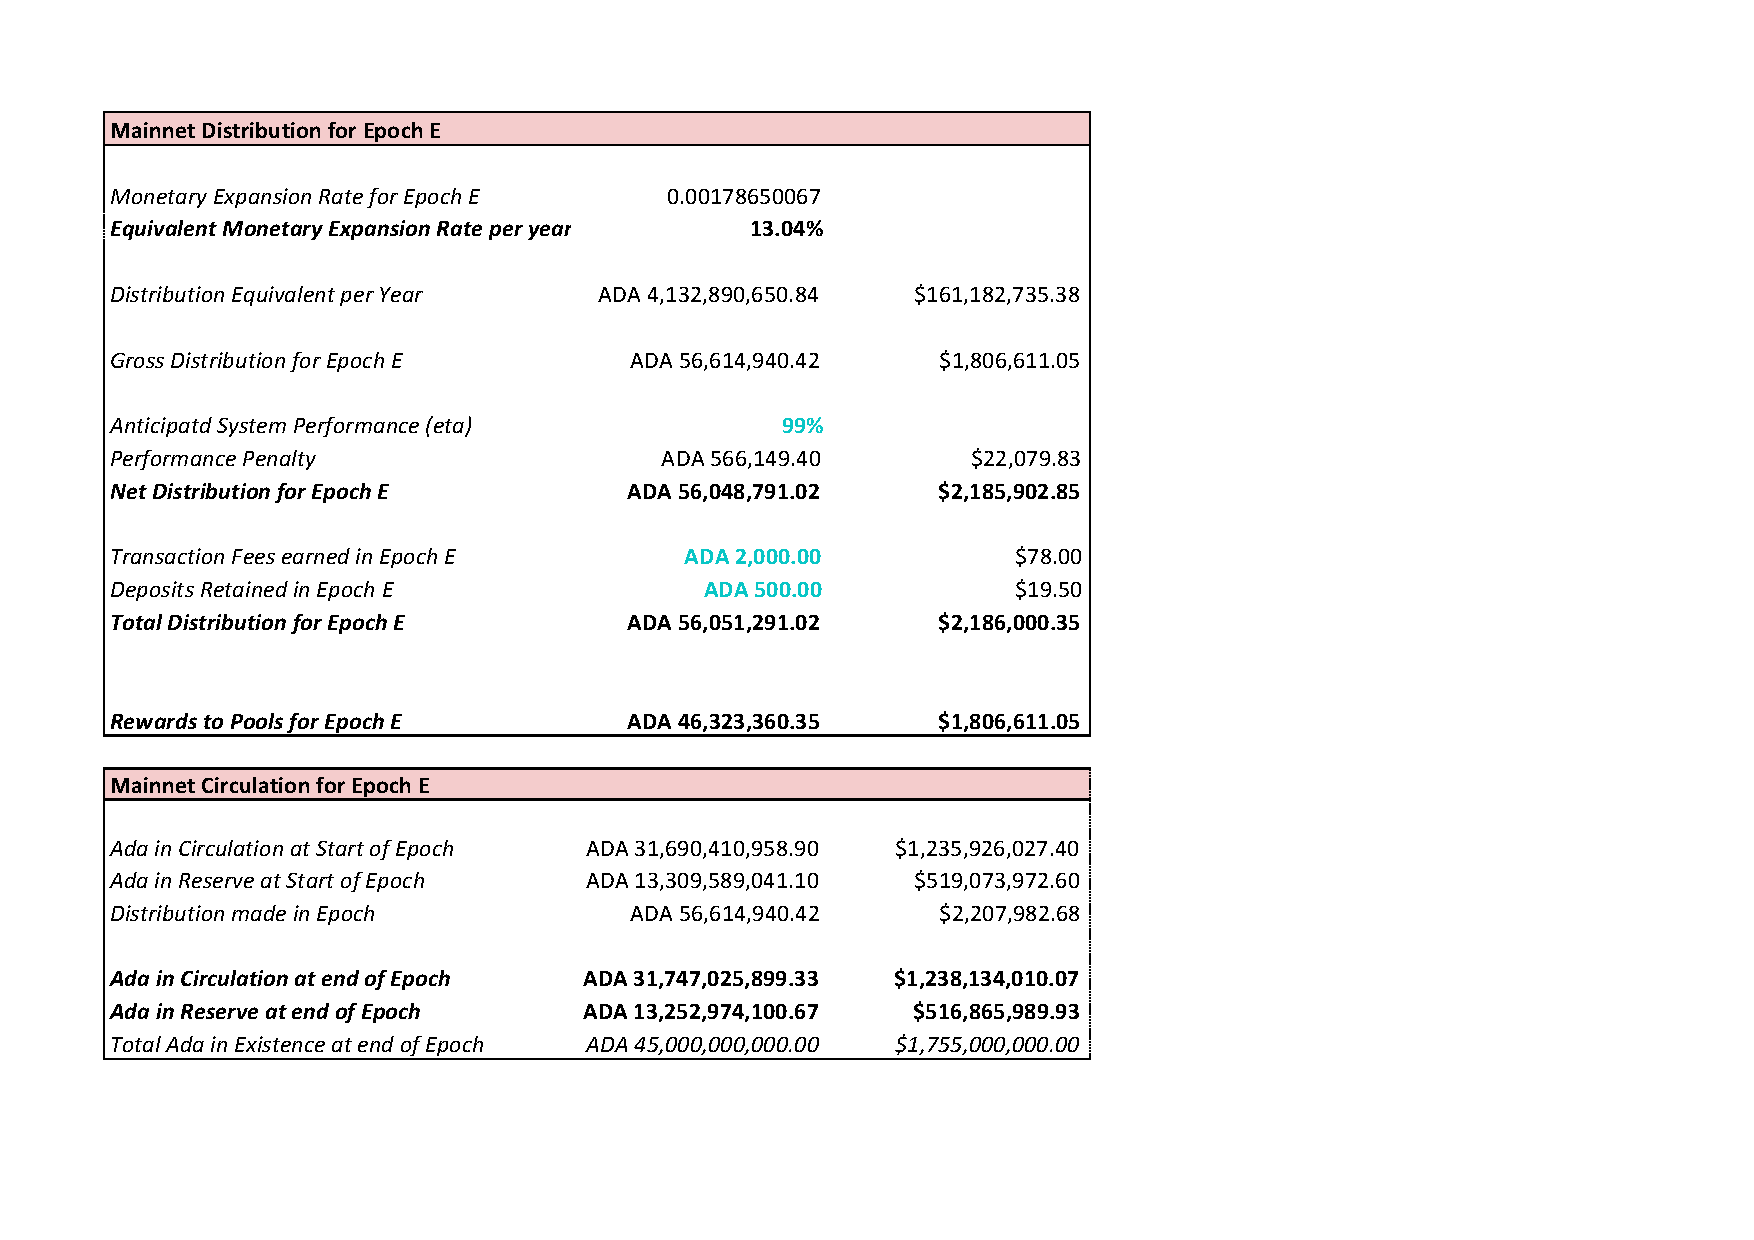
\includegraphics[width=1.6\textwidth]{RCM2.pdf}

\noindent
The upper part of this diagram shows the \ada{} that is distributed for Epoch E, assuming the overall system performance of 99\%,
retained deposits of \ADA{500} and transaction fees of \ADA{2,000}.  The total distribution for the
Epoch is \ADA{56,051,291.02}.  These are reduced by the Treasury Top Slice and the influence factor
to give the rewards that are distributed to the pools of \ADA{46,323,360.35}.
%
The lower part of the diagram shows the \ada{} in circulation and the reserves at the start and end of the Epoch.

\subsubsection*{StakePool Parameters}

\hspace{-0.65in}
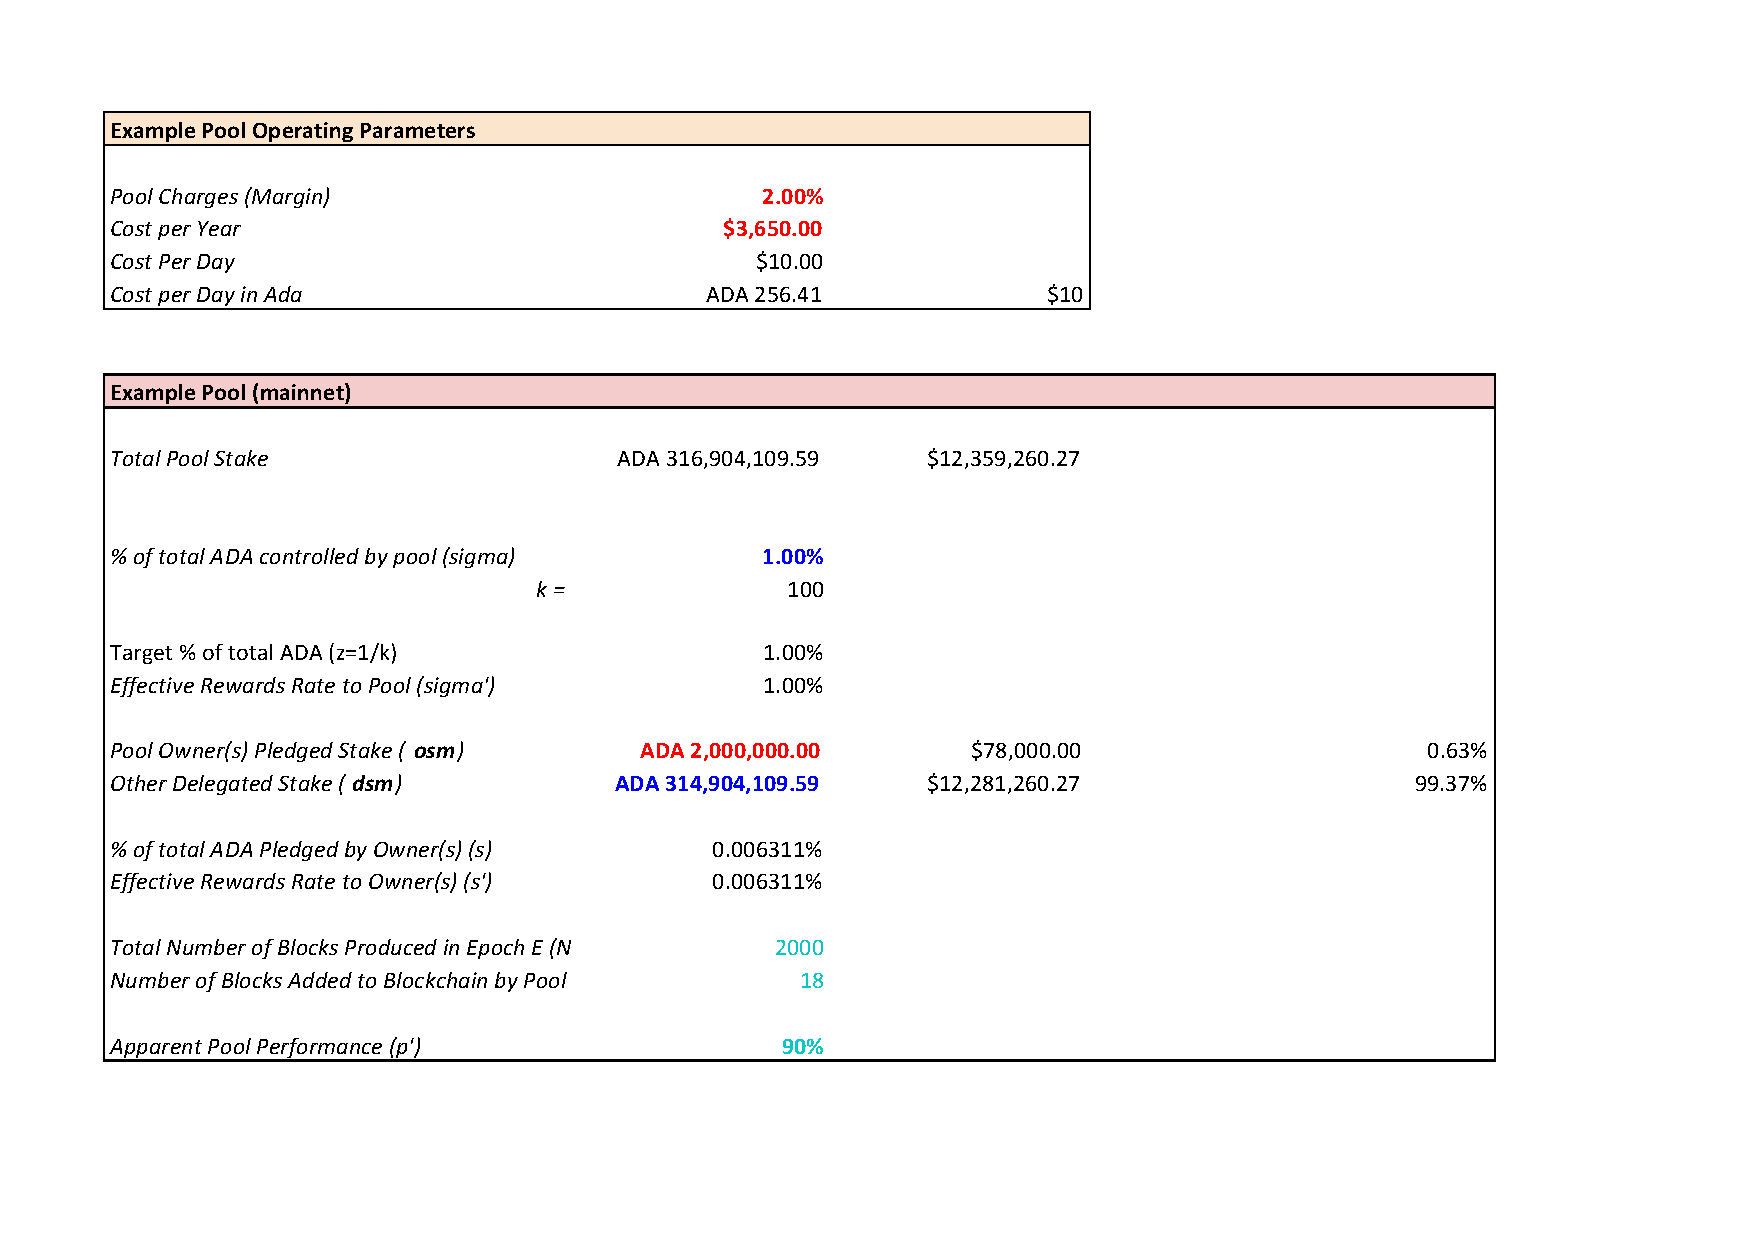
\includegraphics[width=1.25\textwidth]{RCM3.pdf}

\noindent
This diagram shows the StakePool-specific parameters, including the total controlled \ada{} and the
division by owner(s) and delegators.  In the MainNet, 99.37\% of the StakePool \ada{} is owned
by delegators.  As in the simplified scheme, the StakePool receives all of its optimal rewards, since it controls
exactly the required percentage of stake (1.00\%, corresponding to the limit set from
the $k$ parameter).

\subsubsection*{Calculated Rewards}

\hspace{-0.65in}\begin{minipage}{\textwidth}
  \noindent  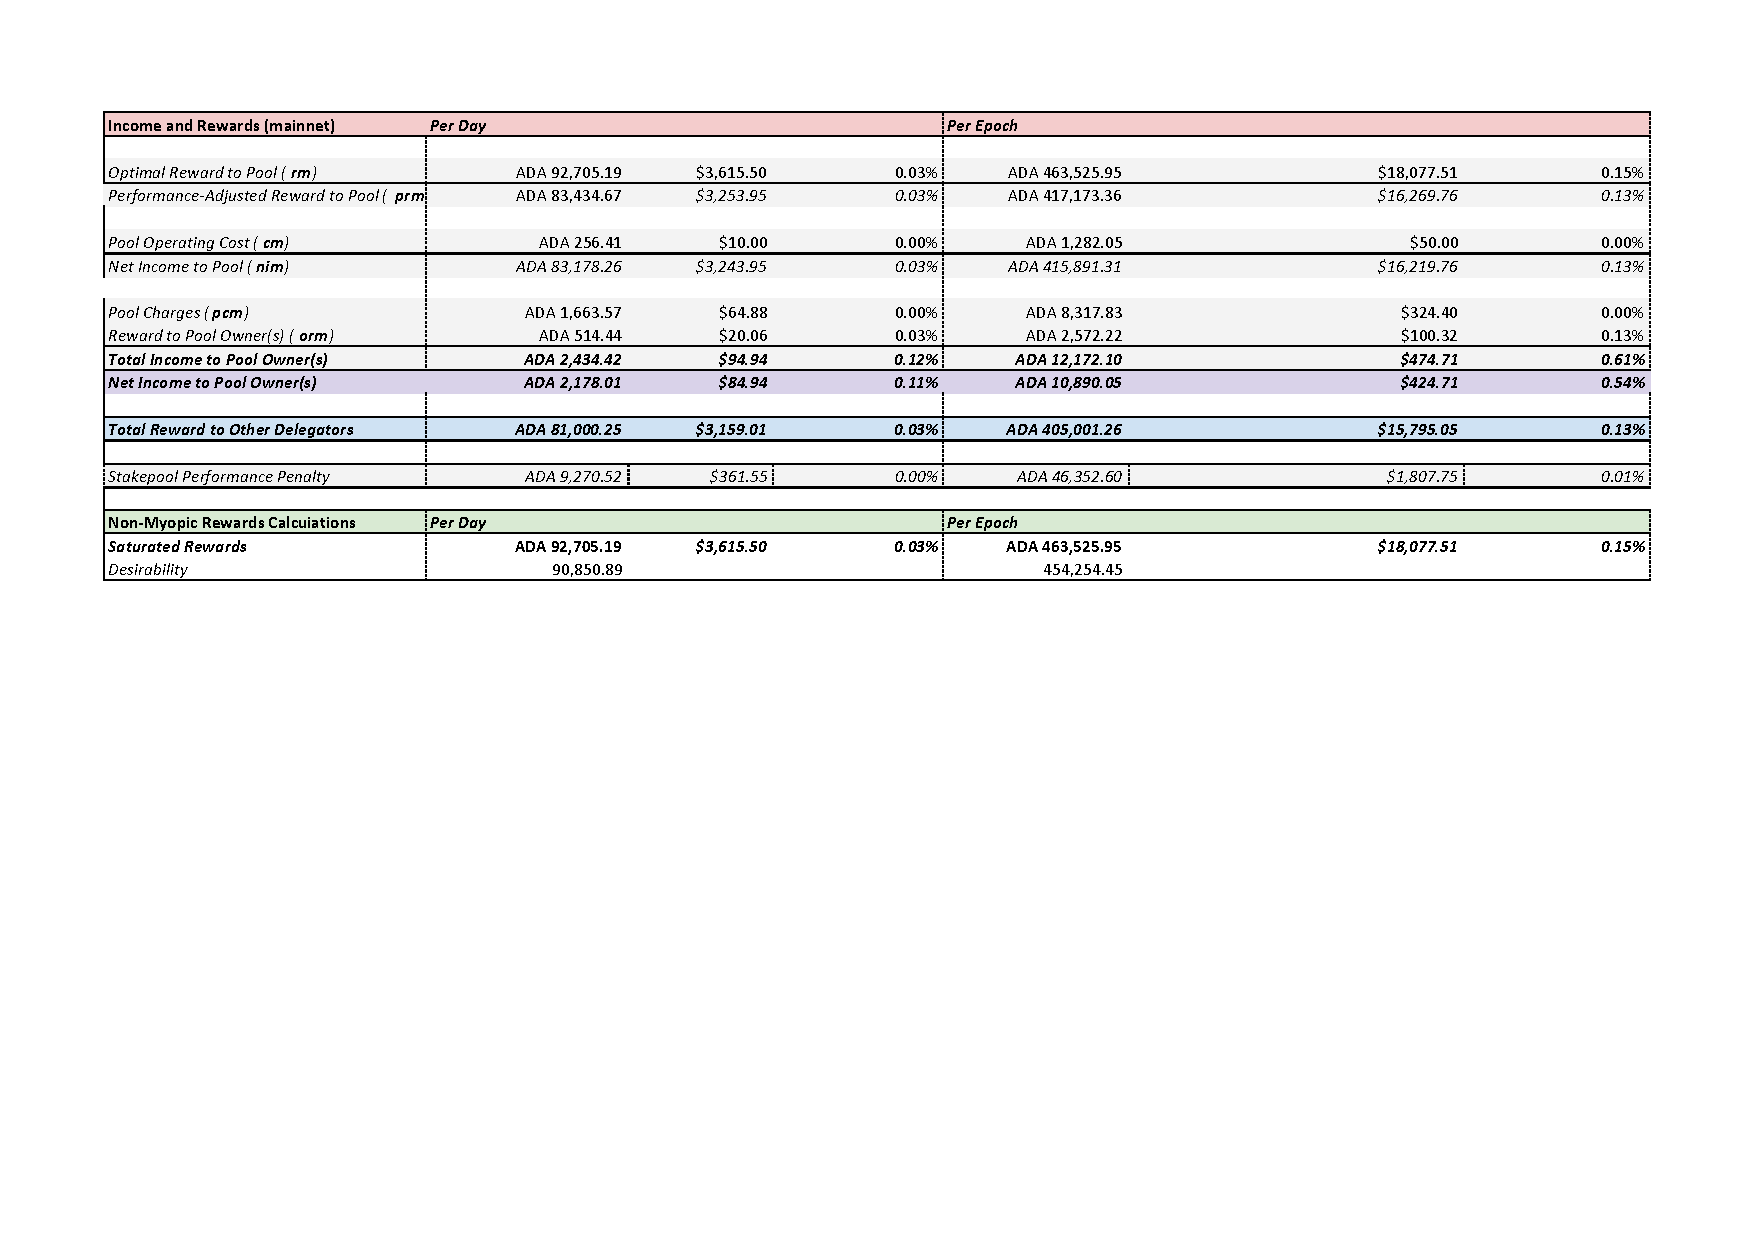
\includegraphics[width=1.2\textwidth]{RCM4.pdf}

  \vspace{-3in}
  \noindent  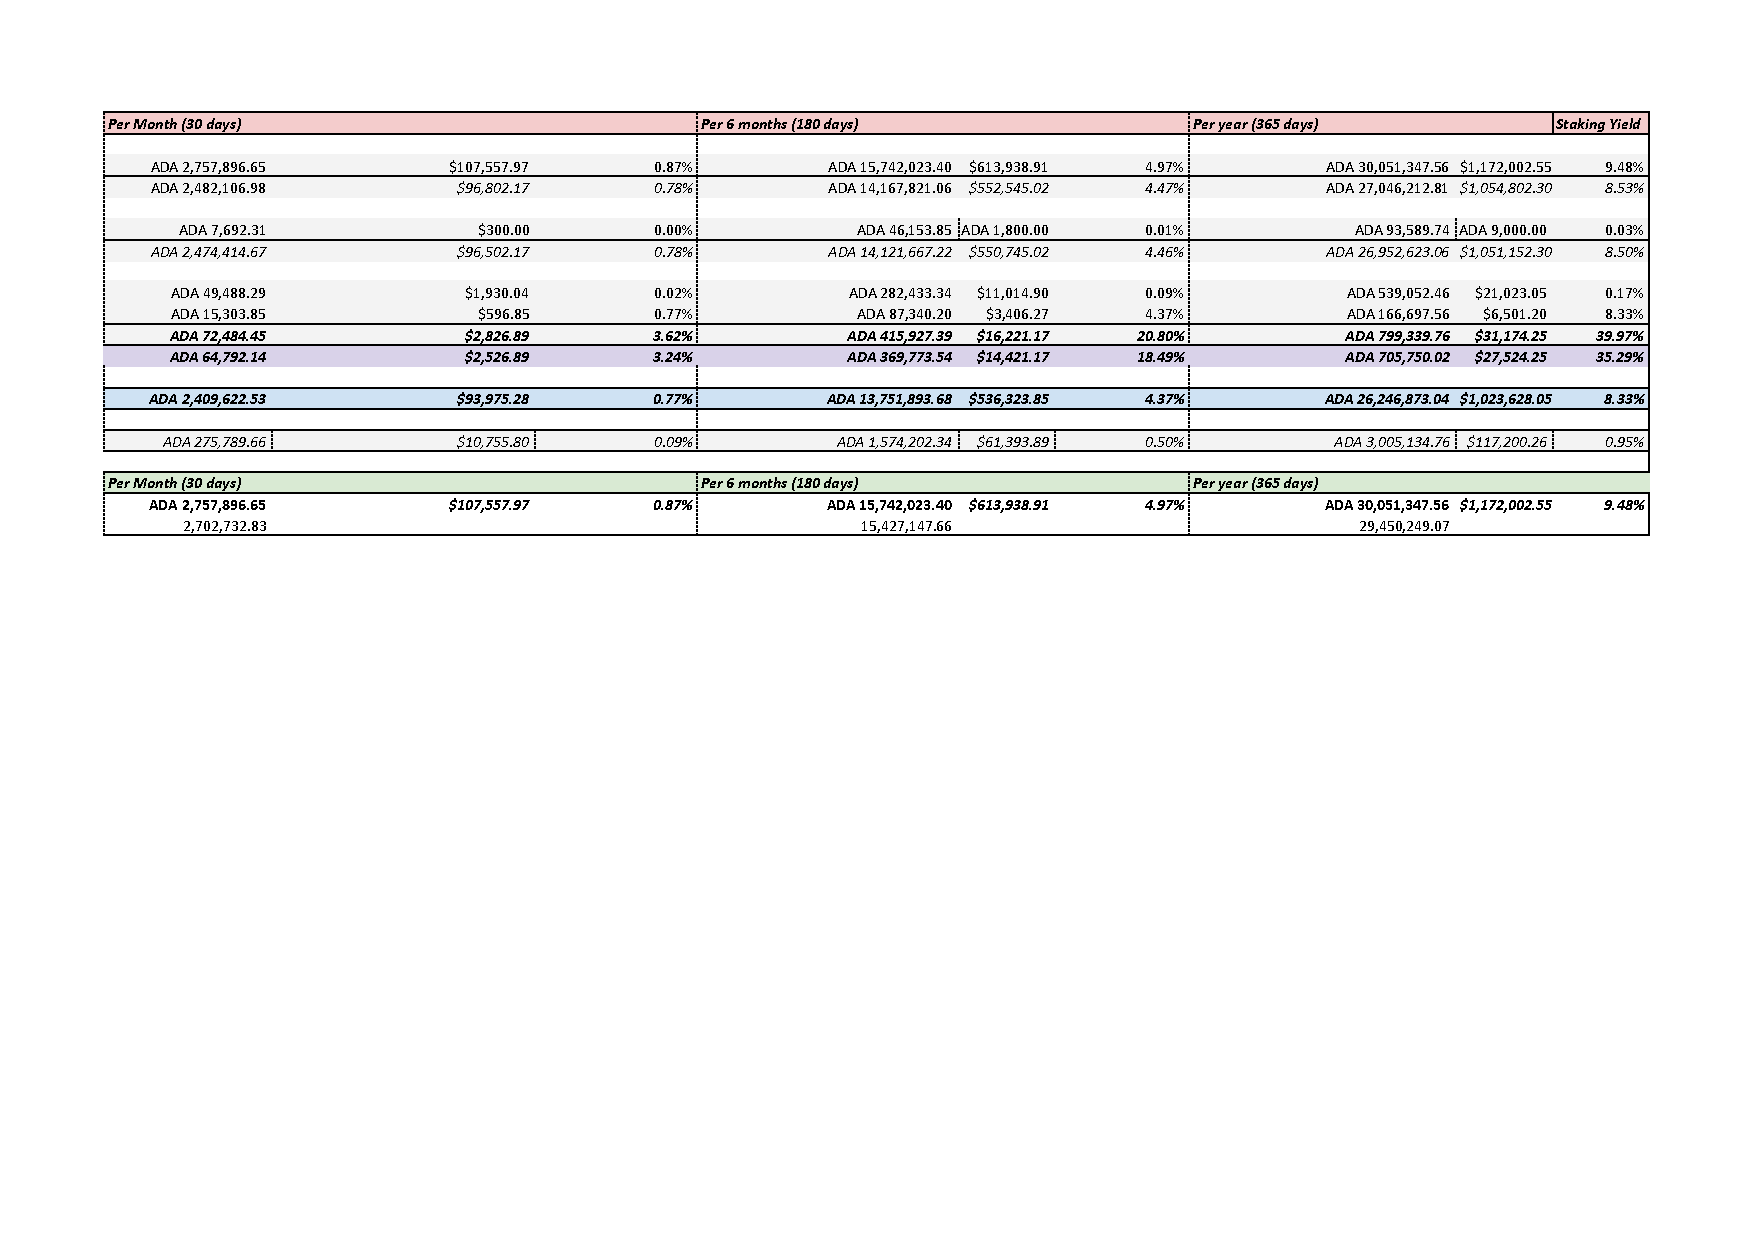
\includegraphics[width=1.2\textwidth]{RCM5.pdf}

  \vspace{-2.8in}
\end{minipage}

\noindent
This diagram shows the corresponding rewards that accrue to the owner(s) and delegators,
plus a calculation of the total income that is received by the owners.  As before, we will assume that the average
and actual gross rewards are the same, i.e. if the StakePool controls 1\% of the total \ada{} in
circulation, it will produce exactly 1\% of the blocks, that it has 100\% performance, and will therefore receive exactly 1\% of the rewards.
In total, the
owners and delegators to this StakePool would receive a net reward that was equivalent to 8.33\% per year
(the ``staking yield''), representing a 17\% better return than with the simplified scheme.
The final rows calculate the \emph{non-myopic} rewards (i.e. long-term rewards that ensure
a stable and well-functioning system).  As described in~\cite{SL-D1}, these values will be used to guide stakeholder behaviour
through a ranking system that will encourage convergence to the $k$ best-performing pools.
For this pool, which is \emph{saturated}, the non-myopic rewards are identical to the \emph{optimal rewards}.
\khcomment{Is this always the case?}
Rewards will be returned as described in Section~\ref{sec:rewards-return}.  In the MainNet, when multiple
owners are involved, this return could be through a multi-signature transaction~\ref{shelley_multisig}, according to an agreed
formula.

\subsubsection*{Delegator Rewards}

\hspace{-0.65in}\begin{minipage}{\textwidth}
  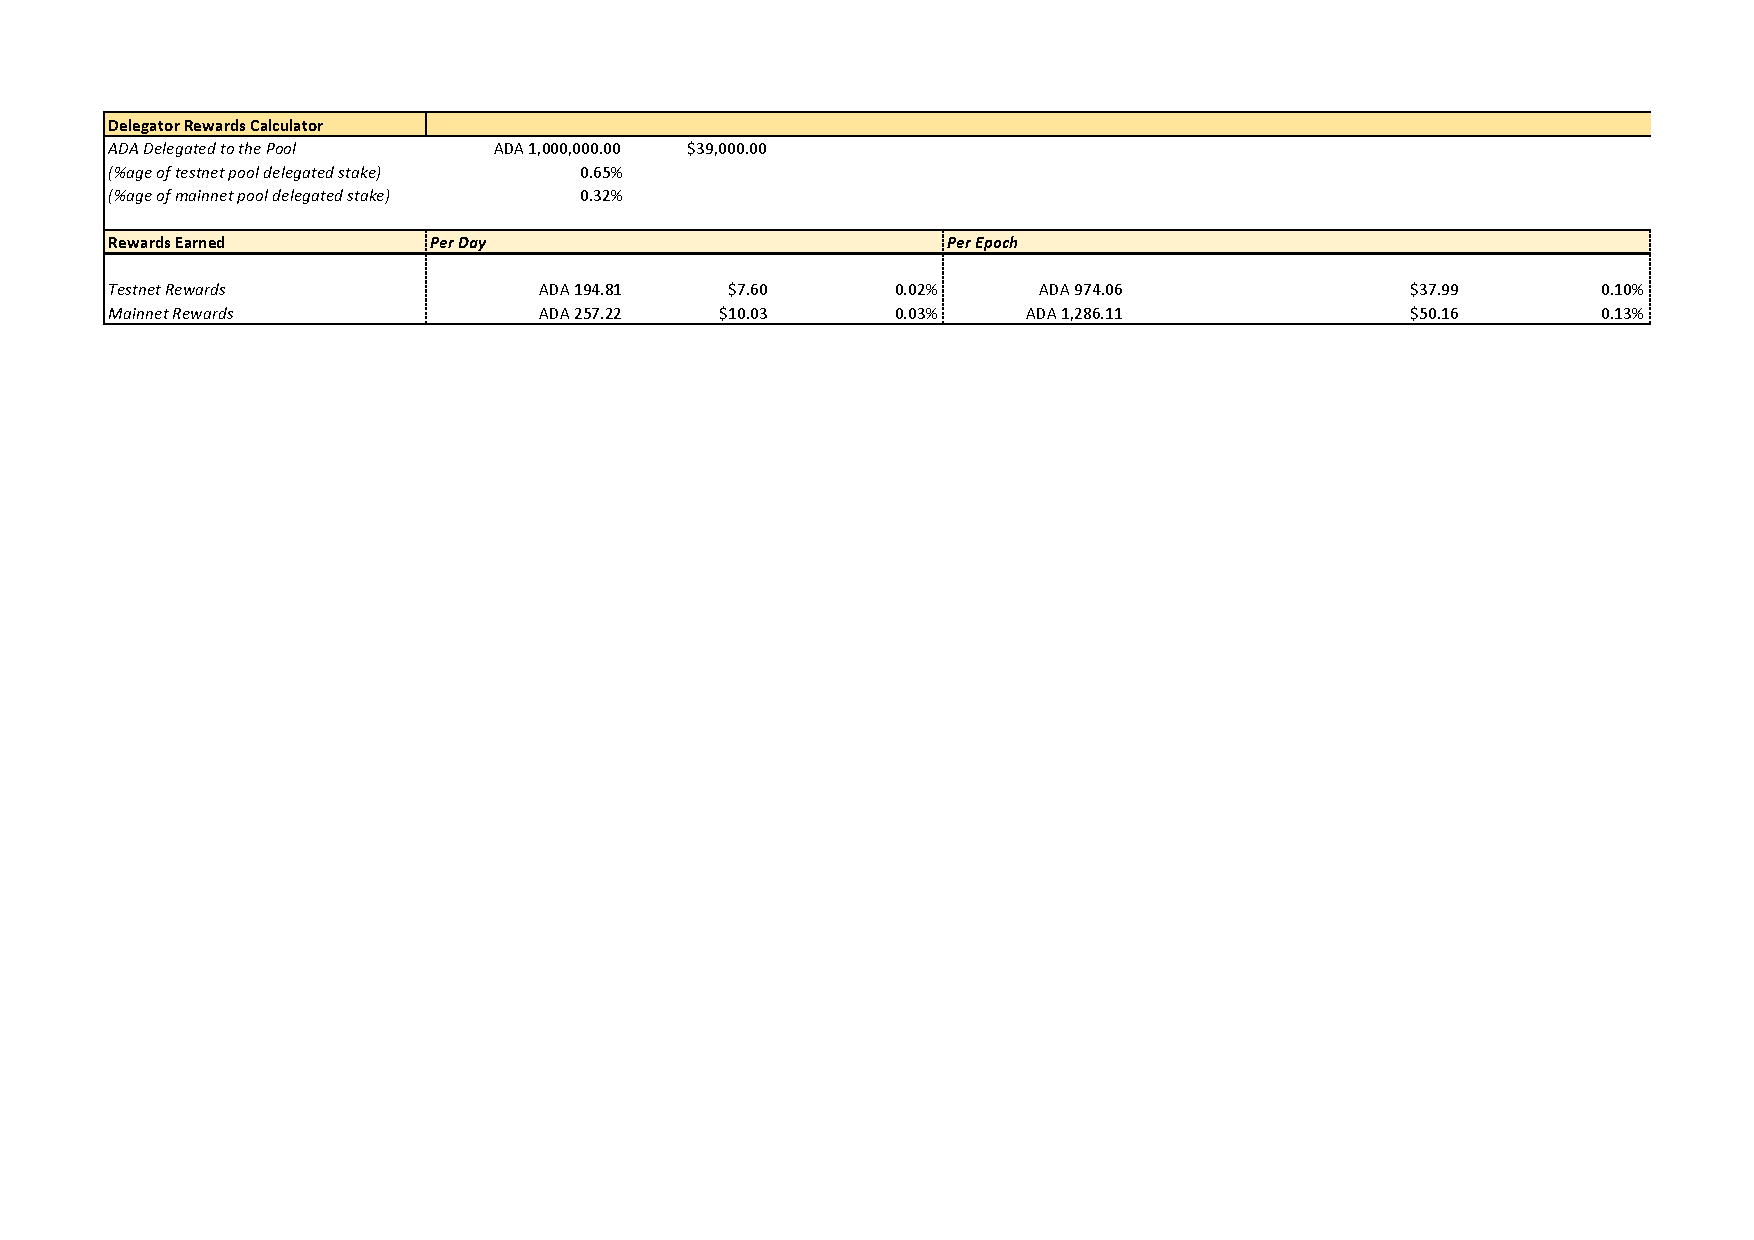
\includegraphics[width=1.2\textwidth]{RCM6.pdf}

\vspace{-3.8in}
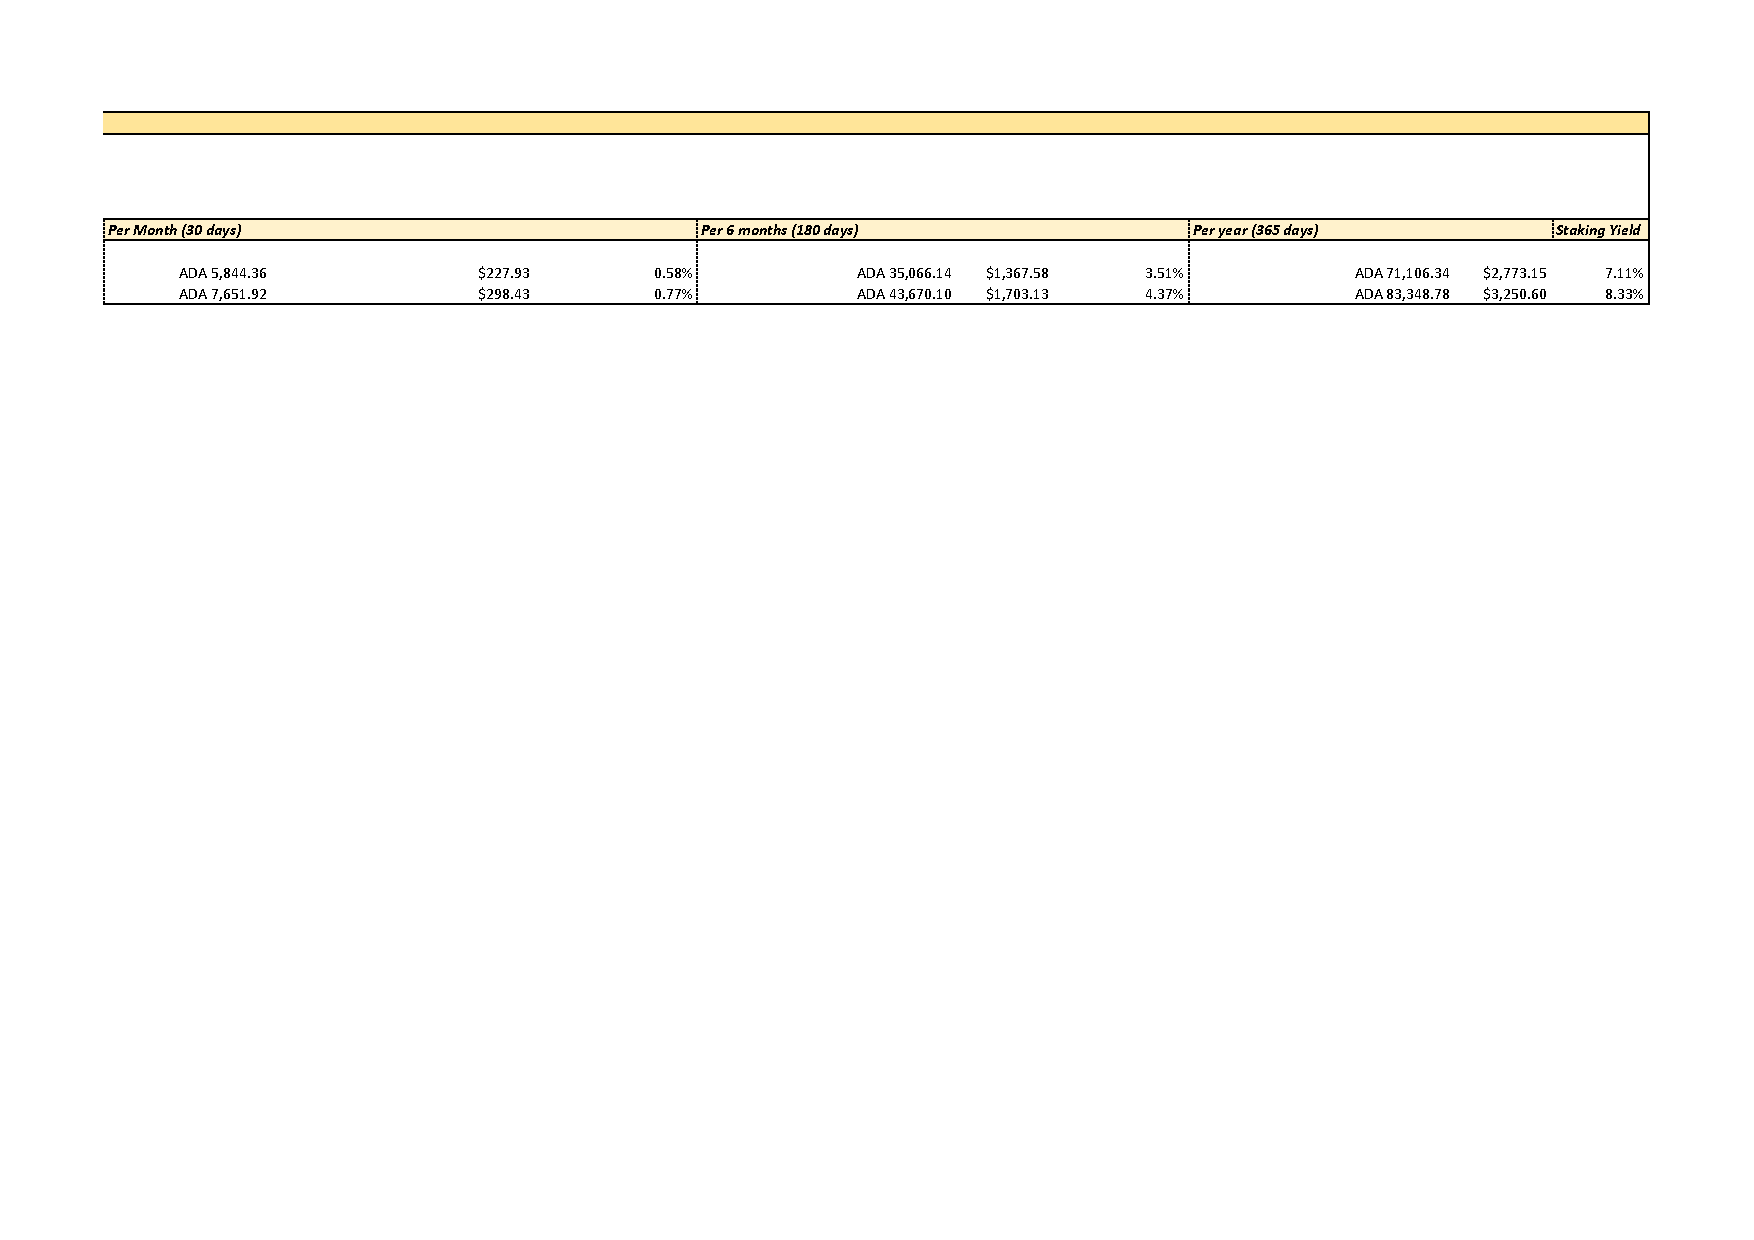
\includegraphics[width=1.2\textwidth]{RCM7.pdf}

  \vspace{-3in}
\end{minipage}

\noindent
This diagram shows the rewards that a stakeholder would receive over time if they delegated \ADA{1,000,000} to
the sample pool under the assumptions used above.  In total, this would represent 0.65\% of the stake
that is delegated to the incentivised TestNet pool, or 0.32\% of the stake that is delegated to the MainNet pool.
Overall, the staking yield would be 7.11\% for the simplified scheme, or 8.33\% for the full scheme, representing
a return of \ADA{70K}-\ADA{80K} over a year.

\clearpage
\subsection{Summary of Differences between the Two Incentives Schemes}
\label{sec:summary}

\begin{figure}[h!]
\begin{center}
\begin{tabular}{||l|p{4cm}|p{4cm}||}
  \hline\hline
  \textbf{Value} & \textbf{Incentivised TestNet} & \textbf{MainNet}
                                              \\\hline
Treasury Top Slice Percentage
& Fixed at 10\%
& Initially set to 10\% but can be changed in future by a community vote
                                              \\\hline
Monetary Expansion Rate per Year
& Fixed at 10\%
& Exponential decay from ~10\%
                                              \\\hline
 Target Number of Stake Pools
                 &
\multicolumn{2}{|p{8cm}||}{
Identical effect, the MainNet settings will be determined based on feedback from the TestNet.
The target is expected to grow over time and may reach around 1000.
It will initially be set low (probably 50 or 100).}
                                              \\\hline
Participation
& Any stakeholder can participate if they hold ADA as of a specific date
& Any stakeholder can participate if they hold ADA
                                              \\\hline
Transaction Fees
& None
& Included in the reward pot
                                              \\\hline
Registration Deposits
& None
& Non-refundable parts included in the reward pot
                                              \\\hline
Influence Factor ($\textit{inf}$)
& None
& Included in calculation, initially set to 0.1
                                              \\\hline
StakePool Performance
& Actual block creation considered
& Directly affects rewards, any ``penalty'' accrues to the treasury
                                              \\\hline
Owner Rewards
& Divided equally amongst multiple Owners
& Owners can decide proportions using a smart contract
                                              \\\hline
ADA that affects rewards
& All ADA that is circulating in the TestNet
& All ADA that is in circulation
                                              \\\hline
Stake pledged by owners
& Assumed to be fully pledged
& % Will be reserved for the duration of the pledge
Affects rewards if not honoured
                                              \\\hline
Epoch duration ($E$)
& Fixed to 1 day
& Set to 5 days initially (but community vote can change)
                                              \\\hline
Treasury Fraction ($T$)
& Fixed at 10\%
& All rewards that are not distributed to the StakePools
                                              \\\hline
\hline
\end{tabular}
\end{center}
\caption{Differences between the Incentivised TestNet and the MainNet}
\end{figure}

\clearpage
\bibliographystyle{habbrv}
\bibliography{references}

\clearpage
\appendix

\section{Summary of Differences in terminology etc. to \cite{delegation_design}}
\label{app:diffs}


\begin{itemize}
\item
  SL-D1 only considers the full incentives calculation, not the simplified one, or how
  rewards are to be transferred to the MainNet.
\item
  SL-D1 does not distinguish the StakePool Operator and Owner(s).
\item
  SL-D1 does not use the terms ``Control'' or ``Distribution''.
\item
  This document uses terminology that is intended to convey the purpose of specific symbols
  in SL-D1.  The main differences are shown below.

  \begin{center}
  \begin{tabular}{||l|l||}\hline\hline
    \textbf{SL-D1} & \textbf{This Document} \\ \hline
  $a_0$ & $\textit{inf}$ \\ \hline
  $\eta$ & $\textit{Perf}_E$ \\ \hline
  $\bar{p}$  & $\textit{Pool}^{\textit{Perf}}$ \\ \hline
  $\rho$ & $\textit{MER}$ \\ \hline
  $s$  & $\textit{Pool}^{\textit{Pledge}}$ \\ \hline
  $s'$  & $\textit{p}^{\%}$ \\ \hline
  $\sigma$ & $\textit{Pool}^{\textit{Perf}}$ \\
  $\sigma'$  & $\textit{s}^{\%}$ \\ \hline
%  $\sigma$  & $\textit{Pool}^{\textit{Tot}}$ \\ \hline
  $\tau$  & $T$ \\ \hline
  $T_{\infty}$  & $\textit{Ada}^{Tot}$ \\ \hline
  $z_0$ & $z$ \\ \hline
\hline
\end{tabular}
\end{center}
\end{itemize}

\end{document}


%%% Local Variables:
%%% mode: latex
%%% TeX-master: t
%%% End:
